\chapter{Resultados}
\label{chap:resultados}

Em vista dos procedimentos teóricos aliados a uma solução computacional, obteve-se os seguintes resultados:
\begin{itemize}
    \item resposta em frequência;
    \item sugestão de notas;
    \item sugestão de acordes;
    \item detecção de transições rítmicas;
    \item implementação da transformada wavelets;
    \item transcrição de notas ao longo do tempo;
    \item transcrição automática de acordes ao longo do tempo;
    \item extração da tonalidade.
\end{itemize}

% Comentar cada item e o fundamento teórico por trás de cada um

\section{Resposta em Frequência e Sugestões de Notas e Acordes}

Para a demonstração dos resultados dos procedimentos \ref{subsec:procedimento_1}, \ref{subsec:procedimento_2}, \ref{subsec:procedimento_3}, \ref{subsec:procedimento_4}, \ref{subsec:procedimento_5}, \ref{subsec:procedimento_6}, \ref{subsec:procedimento_8}, \ref{subsec:procedimento_9} e \ref{subsec:procedimento_10} e ciclos de desenvolvimento \ref{subsec:ciclo_1}, \ref{subsec:ciclo_2}, \ref{subsec:ciclo_3}, \ref{subsec:ciclo_4}, \ref{subsec:ciclo_7}, \ref{subsec:ciclo_9}, \ref{subsec:ciclo_11} e \ref{subsec:ciclo_12} foram feitos experimentos\footnote{Nesse trabalho contextualizado na computação musical chama-se de experimento o procedimento de verificar saídas da solução computacional dada um conjunto de entradas. Para tal há condições pré-determinadas de ambiente acústico e forma de processamento para que os mesmos possam ser realizados por terceiros.} com todas as possibilidades de reconhecimento de acordes proporcionados pelo sistema. Todavia serão detalhados e comentados somente 4 pois para os outros equivalem as mesmas considerações. O resumo dos resultados dos outros acordes estará presente na tabela que se segue logo após.


\subsection{Pré-condições dos Experimentos}
\label{sec:precondicoes}

No que tange às pré-condições foram levados em conta:
\begin{itemize}
    \item teclado yamaha E413 com som de piano para a execução dos acordes;
    \item somente tríades (3 notas) tocadas;
    \item o software Audacity \footnote{http://www.audacity.sourceforge.net} foi utilizado para gravação;
    \item o microfone convencional interno do $notebook$ foi utilizado para aquisição dos sinais de áudio;
    \item o ruído de fundo estava com uma grandeza por volta de 45 db;
    \item a taxa de amostragem do sinal foi configurada em 44100 Hz;
    \item gravação do áudio no formato de arquivo .wav em codificação 16 pcm.
\end{itemize}


As tríades de acordes foram executadas com base na nota central $C4$ que possui o valor de aproximadamente 261,6 Hz. A figura \ref{fig:teclado} ilustra as regiões e limites usados \cite{teclado}:

\begin{figure}[h]
	\centering
		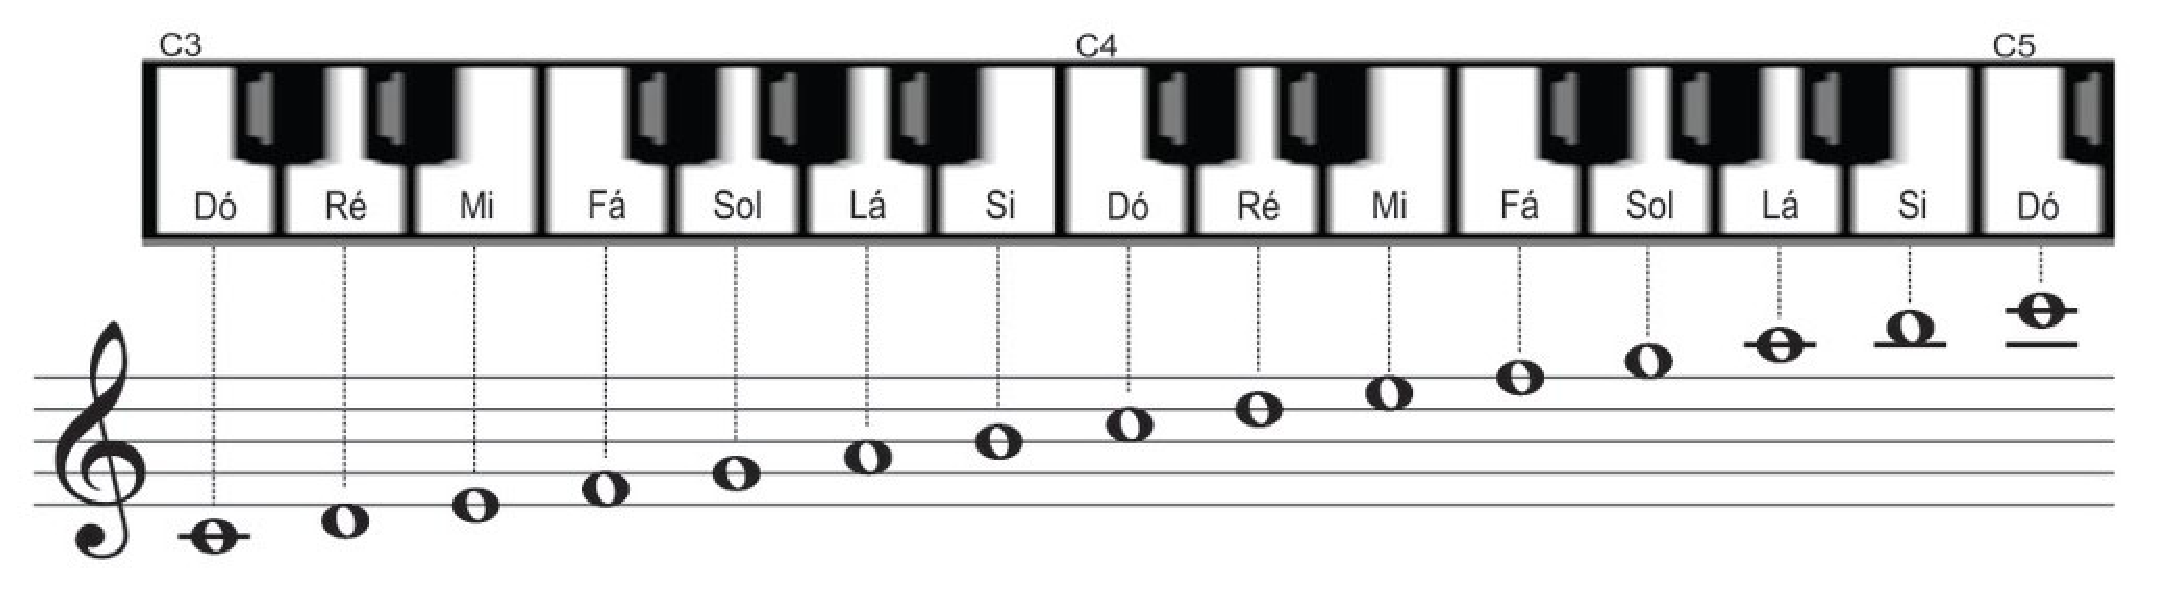
\includegraphics[keepaspectratio=true,scale=0.4]{figuras/teclado-tcc1.eps}
	\caption{Teclado ilustrativo para execução dos acordes.}
  \label{fig:teclado}
\end{figure}

O processo de execução do experimento foi dividido em 4 etapas. A primeira relativa a gravação do acorde tocado no teclado via microfone convencional interno do $notebook$. A segunda é a exportação do som no formato de arquivo .wav pelo software audacity. A terceira etapa é a introdução do arquivo na entrada do sistema de detecção de acordes. A última atividade é a classificação do arquivo digital num acorde. A figura \ref{fig:processo} ilustra o processo esquematizado.

\begin{figure}[h]
	\centering
		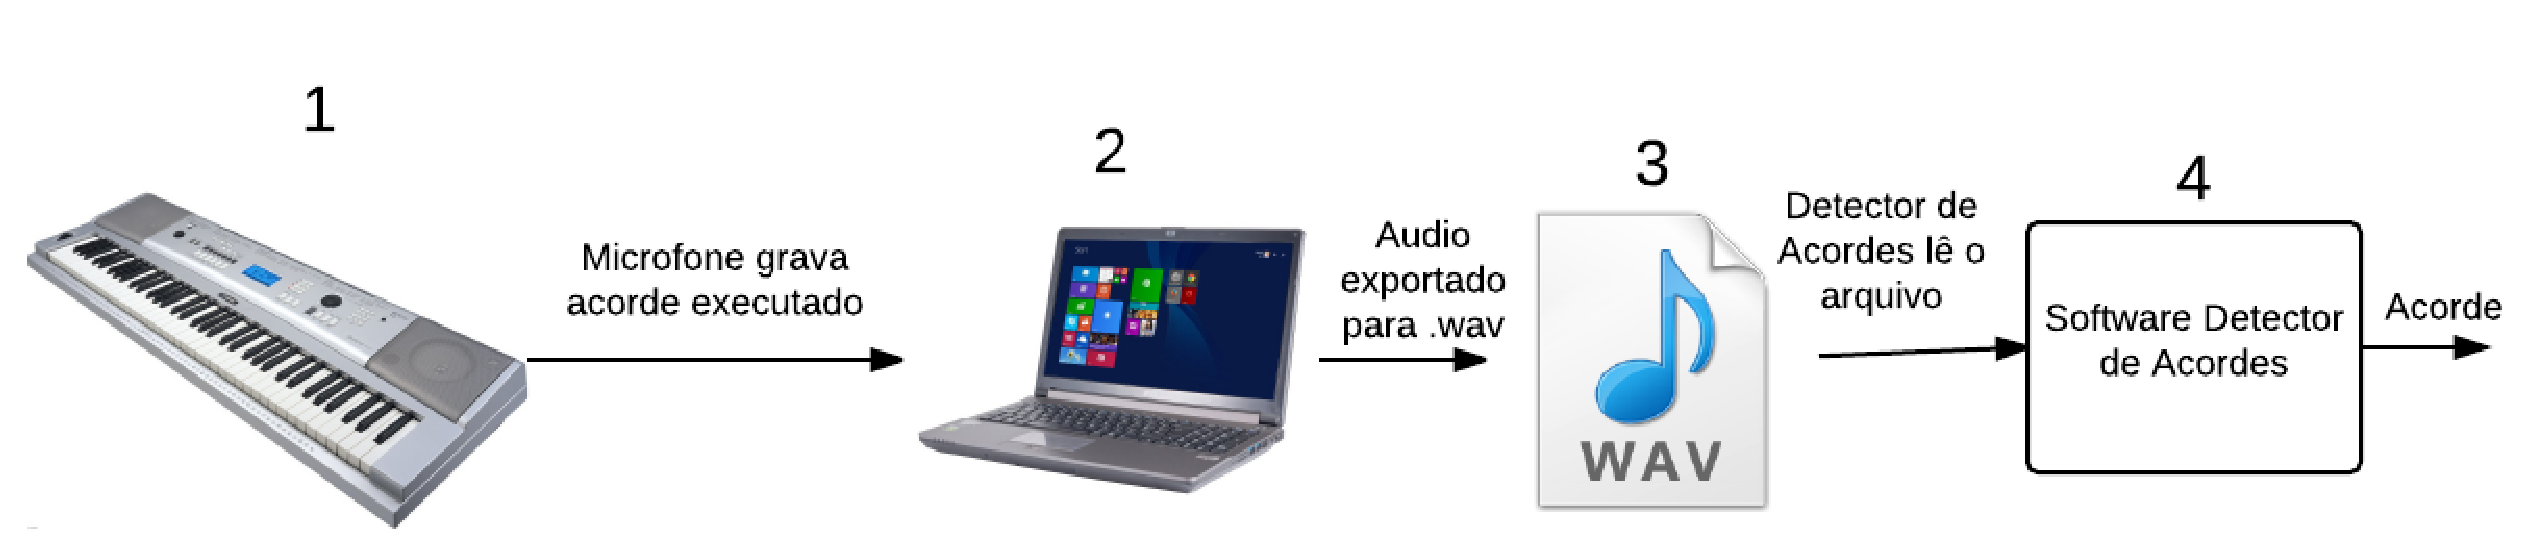
\includegraphics[keepaspectratio=true,scale=0.35]{figuras/processo_experimento.eps}
	\caption{Processo ilustrativo da execução dos experimentos.}
  \label{fig:processo}
\end{figure}


\subsection{Experimento 1 - Acorde $CM$}
\label{sec:experimento1}

Nesse experimento foi tocado a tríade $Dó$ (baixo e tônica), $Mi$ e $Sol$ equivalente ao acorde $CM$. A tríade foi tocada ao mesmo tempo e com a mesma força para todas as notas.

Segue os gráficos resultantes:

\begin{figure}[h]
	\centering
		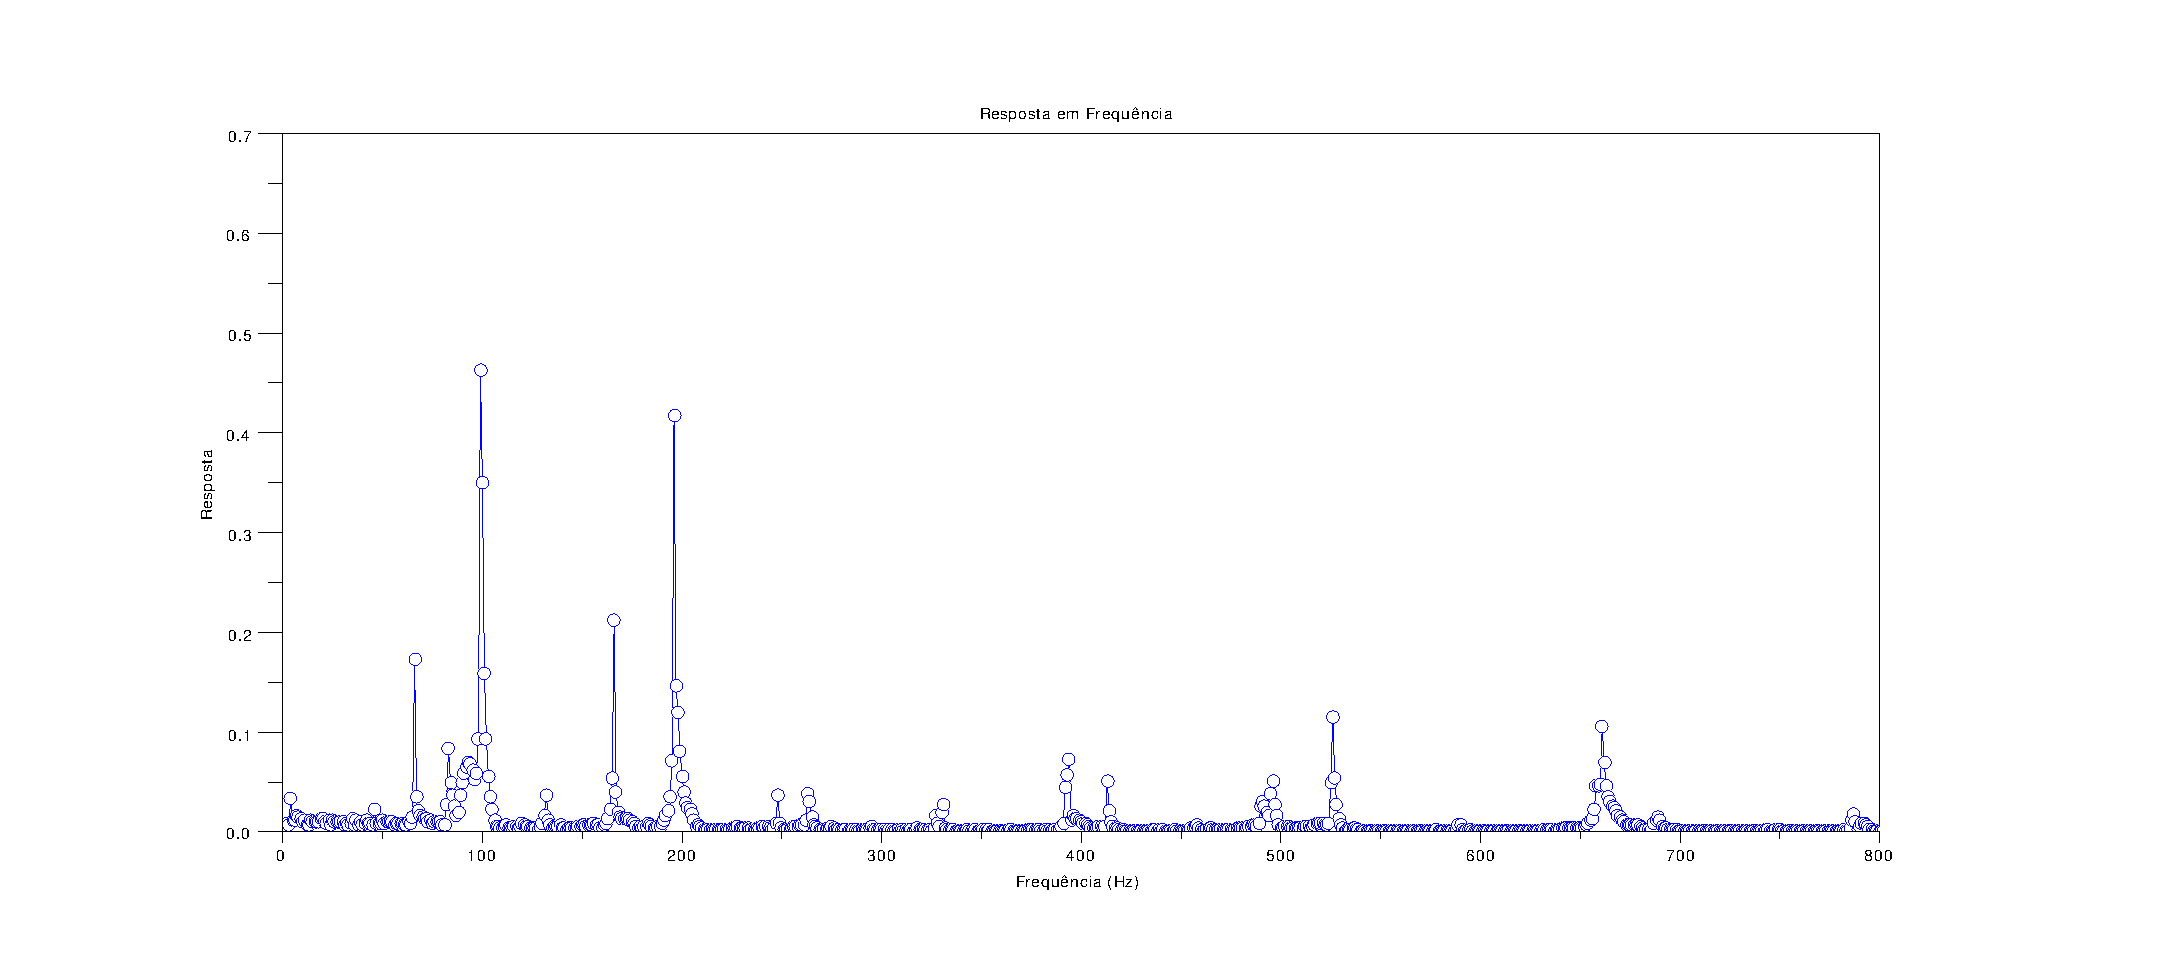
\includegraphics[keepaspectratio=true,scale=0.49]{figuras/CM/fft_cm.eps}
	\caption{Gráfico da resposta em frequência para a gravação do acorde $CM$.}
  \label{fig:espectro_CM}
\end{figure}

\begin{figure}[h]
	\centering
		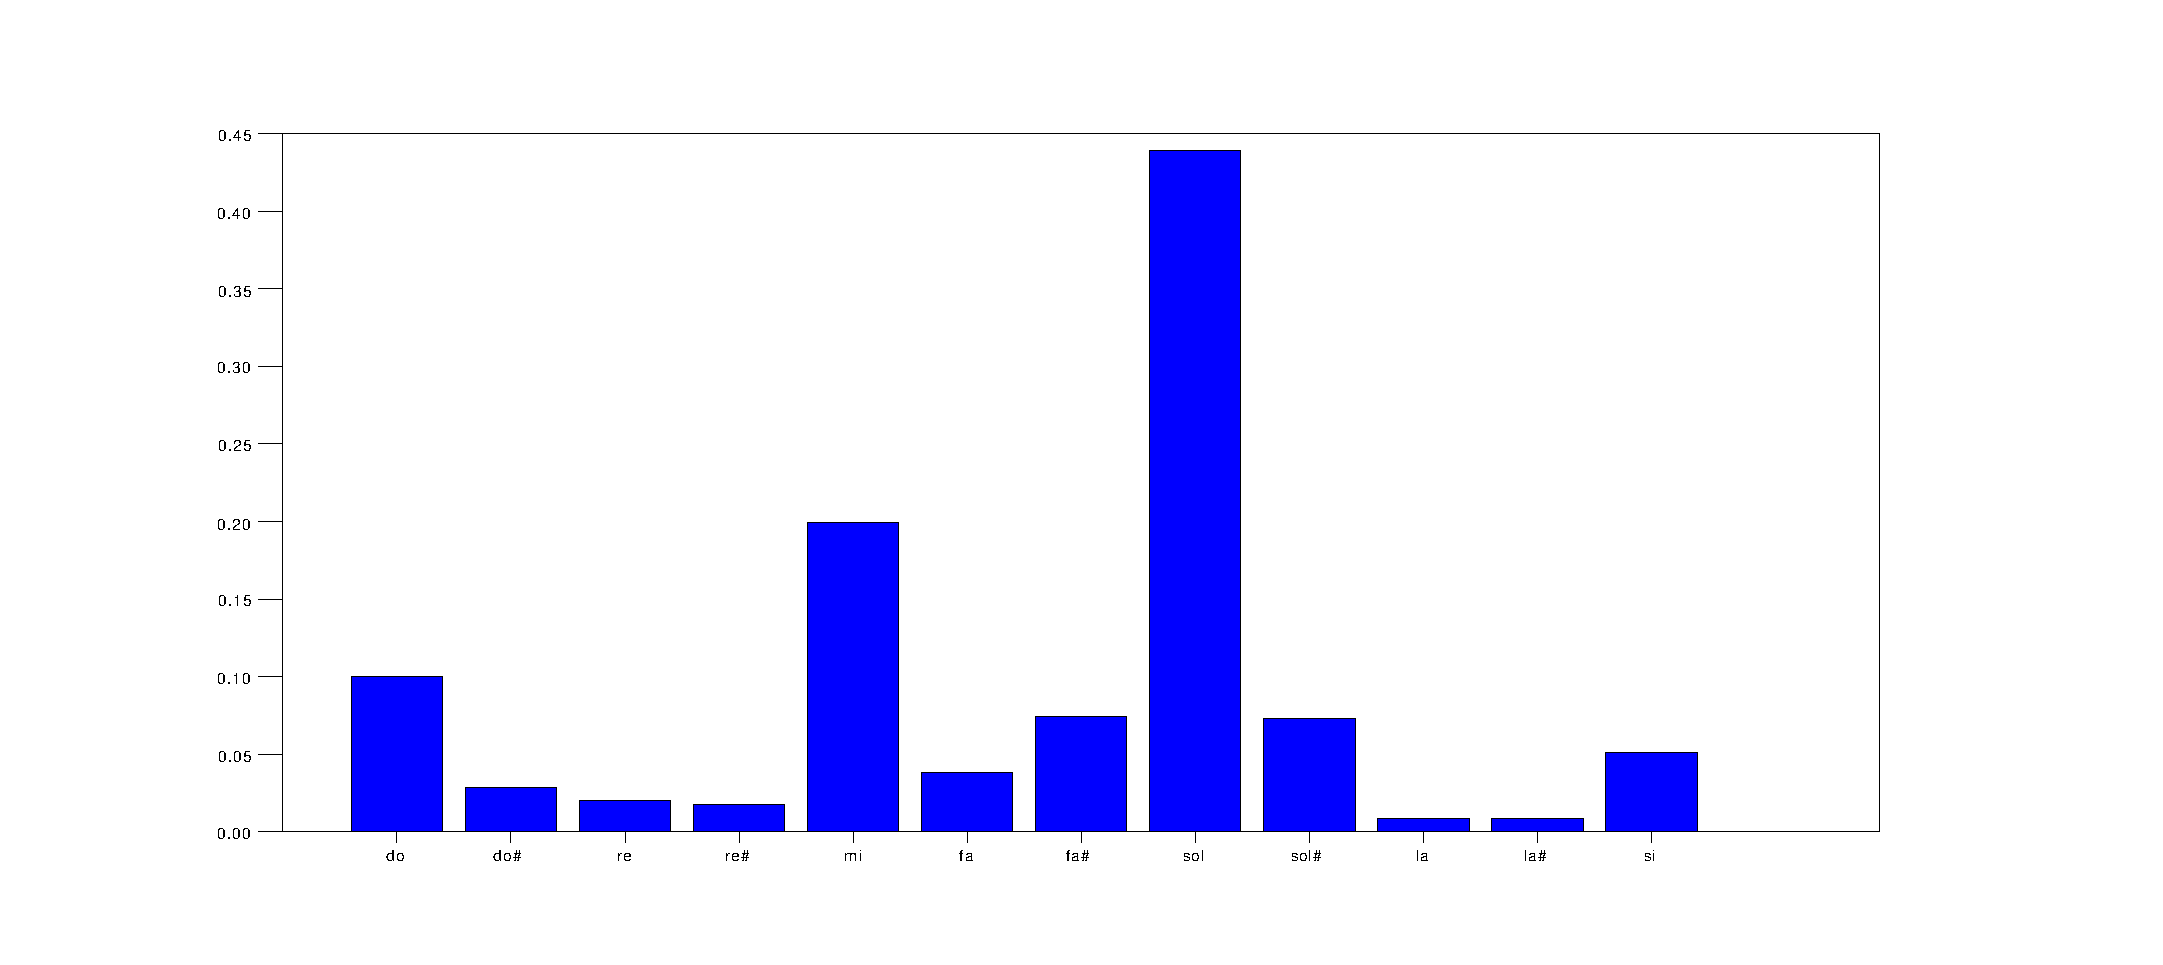
\includegraphics[keepaspectratio=true,scale=0.49]{figuras/CM/notas_cm.eps}
	\caption{Gráfico de sugestão de notas para a gravação do acorde $CM$.}
  \label{fig:notas_CM}
\end{figure}

\begin{figure}[h]
	\centering
		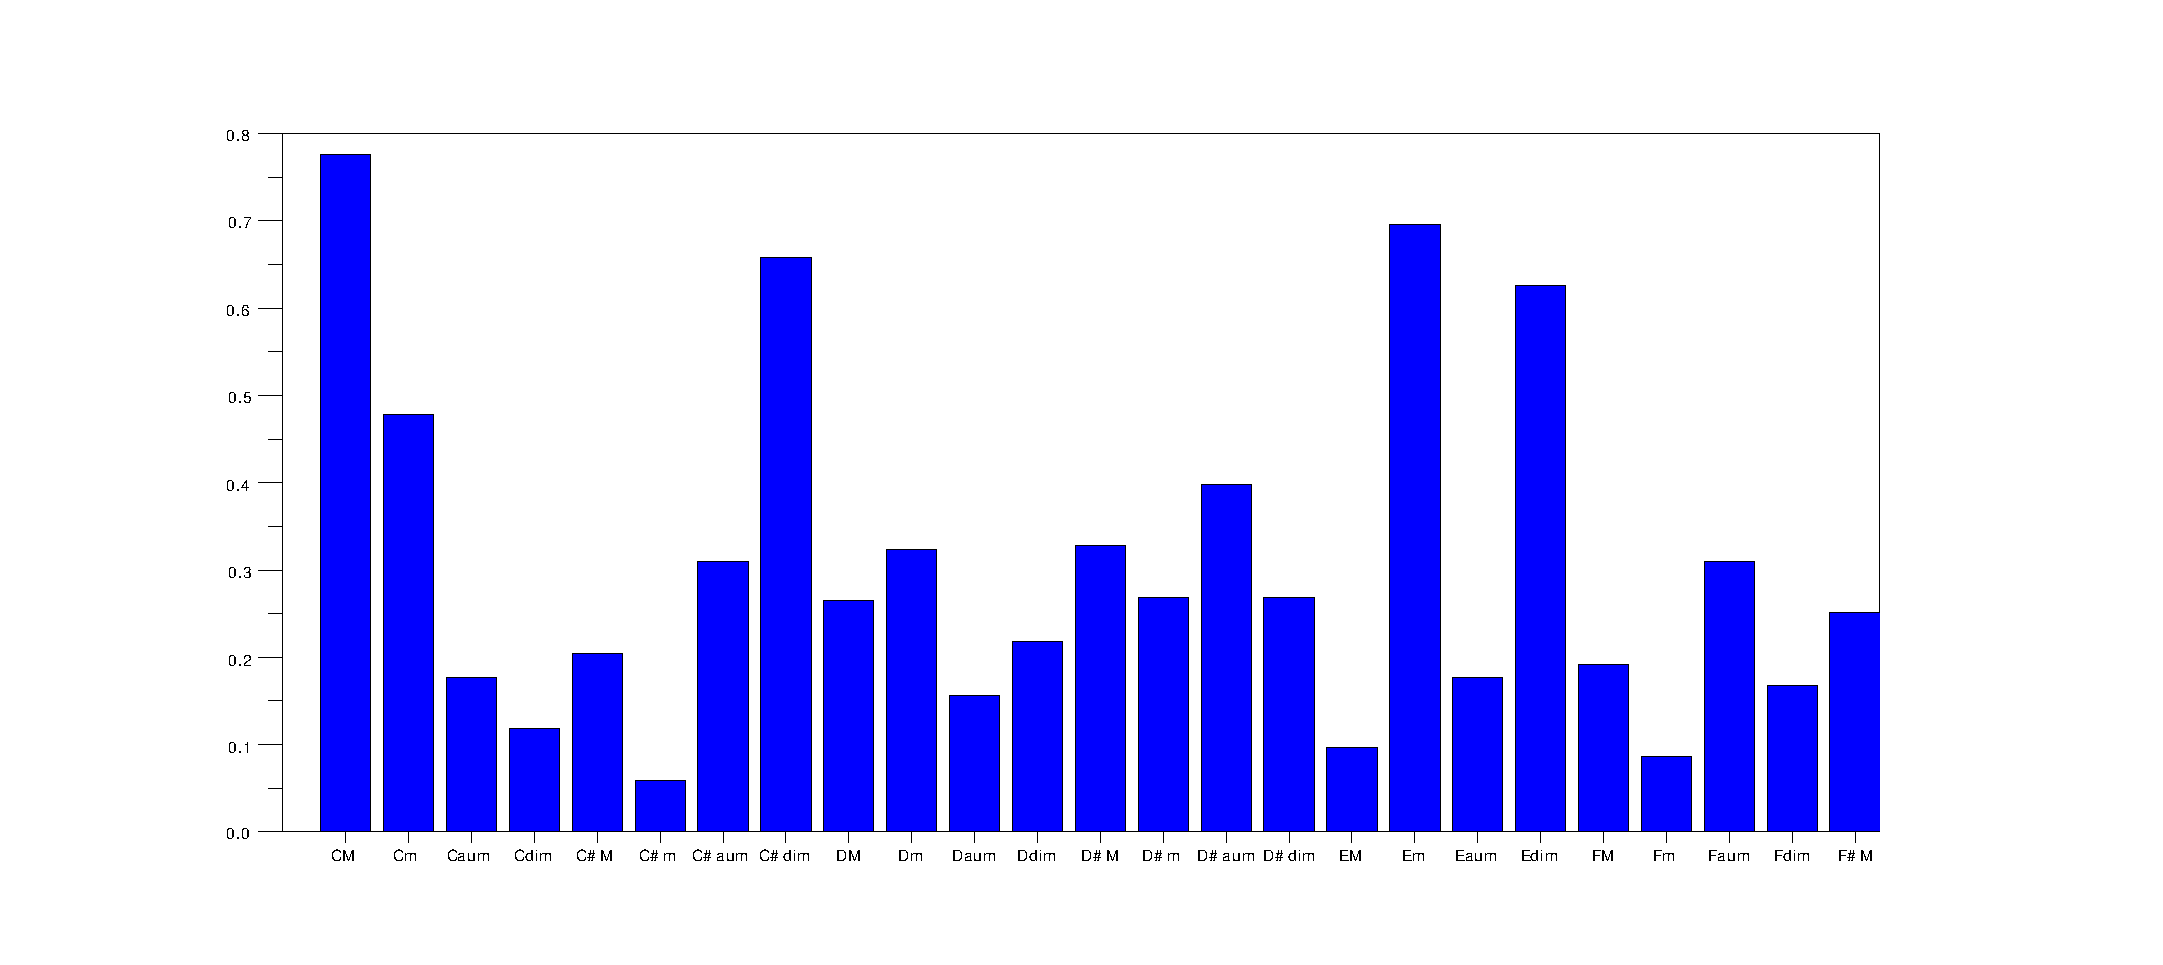
\includegraphics[keepaspectratio=true,scale=0.45]{figuras/CM/acordes_1_cm.eps}
		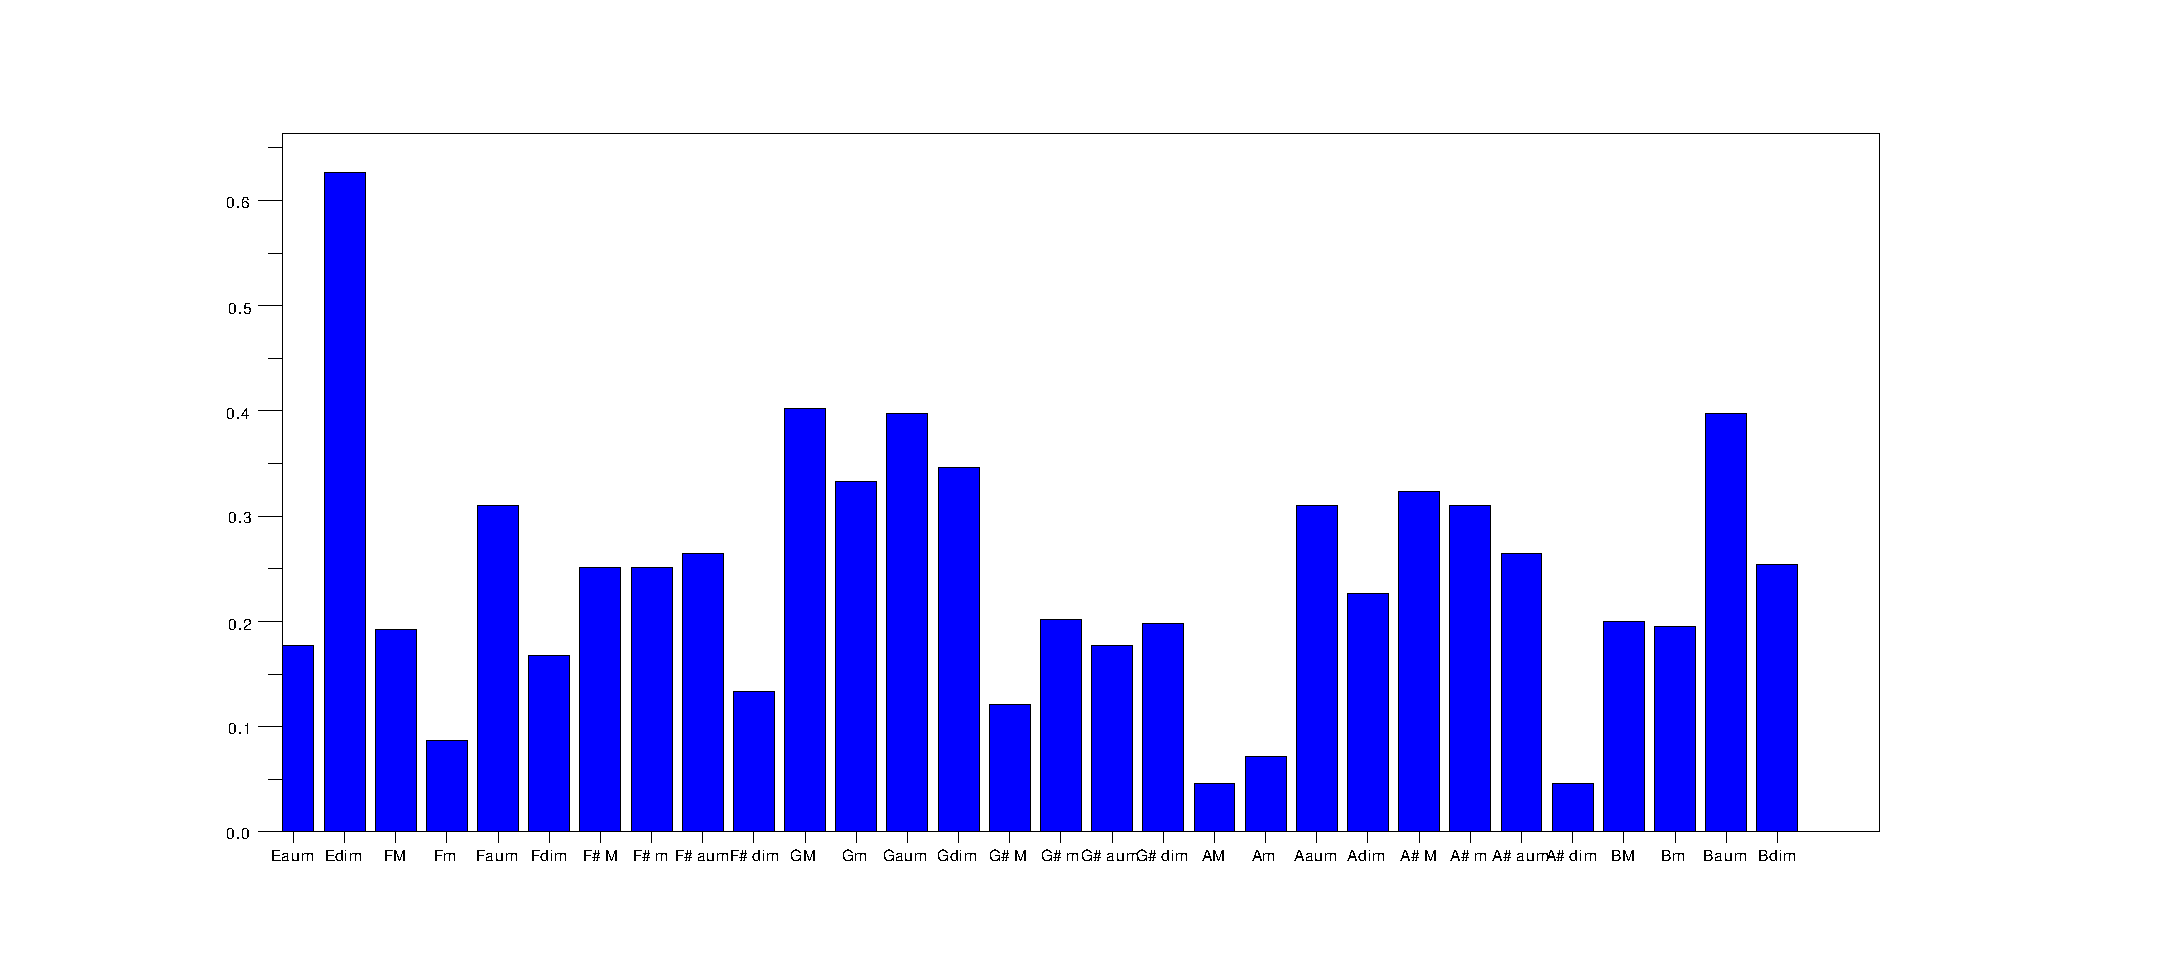
\includegraphics[keepaspectratio=true,scale=0.45]{figuras/CM/acordes_2_cm.eps}
	\caption{Gráficos de sugestão de acordes a gravação do acorde $CM$.}
  \label{fig:acordes_CM}
\end{figure}

Do resultado da primeira camada de processamento é gerado o gráfico da figura \ref{fig:espectro_CM}. Esse gráfico diz respeito a natureza da composição do sinal em senoides em termos de transformada de fourier. O primeiro pico, no valor de 294 Hz, é relativo a nota $Dó$. O segundo pico, no valor de 371 Hz, é relativo a nota $Mi$. O terceiro pico, no valor de 441 Hz, é relativo a nota $Sol$. Os picos seguintes são relativos aos harmônicos dessas três notas.

Do resultado da segunda camada de processamento é gerado gráfico da figura \ref{fig:notas_CM}. É possível perceber nele que as notas $Dó$, $Mi$ e $Sol$ são as que mais possuem energia ou, no ponto de vista de sugestão, as mais sugeridas. De certa forma um dos fatores que contribuiram das notas $Dó$ e $Sol$ ser de maiores energias foi devido a presença dos harmônicos.

Do resultado da terceira camada de processamento são gerados os gráficos da figura \ref{fig:acordes_CM}. Essa camada é relativa ao resultados das sugestões de acordes musicais. É perceptível ver a presença da alta sugestão do acorde $CM$.

\subsection{Experimento 2 - Acorde $Dm$}
\label{sec:experimento2}

Nesse experimento foi tocado a tríade $Ré$ (baixo e tônica), $Fá$ e $Lá$ equivalente ao acorde $Dm$. A tríade foi tocada ao mesmo tempo e com a mesma força para todas as notas.

Segue os gráficos resultantes:

\begin{figure}[h]
	\centering
		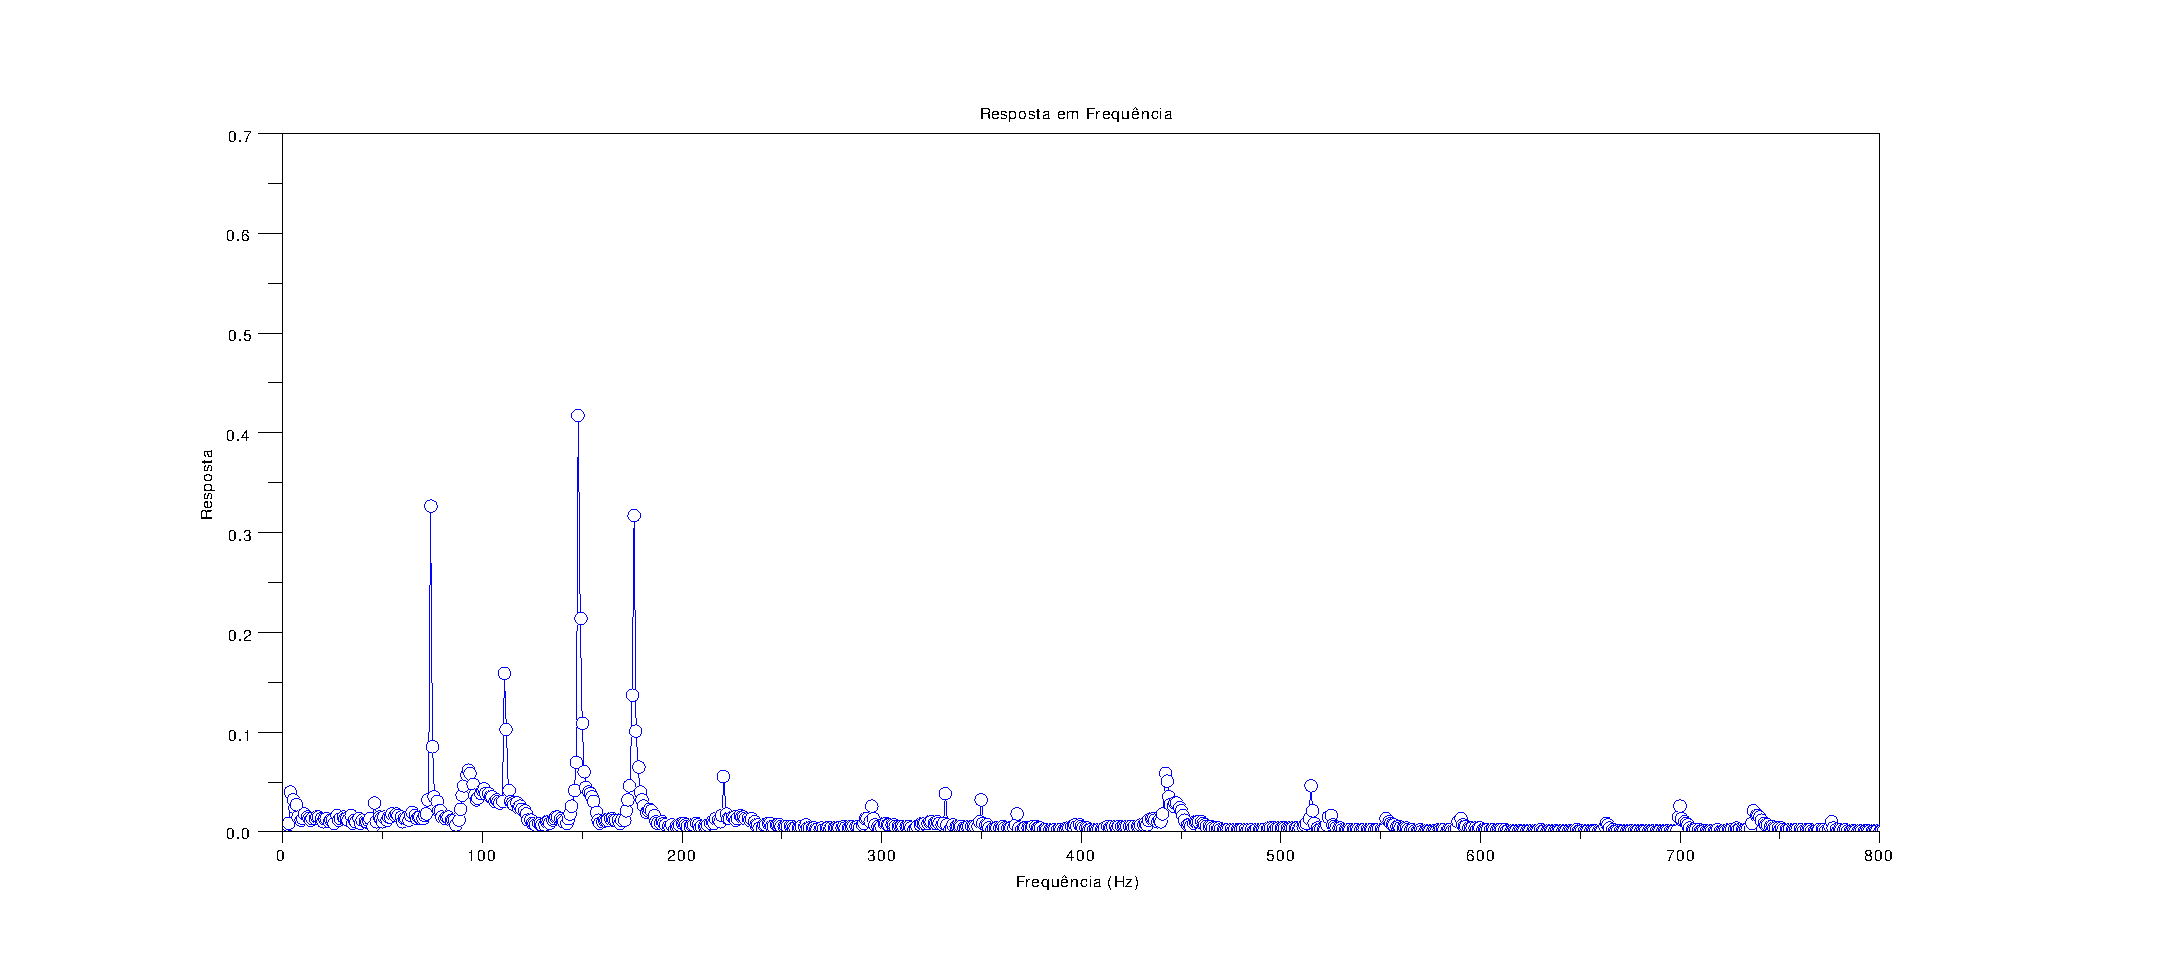
\includegraphics[keepaspectratio=true,scale=0.49]{figuras/Dm/fft_Dm.eps}
	\caption{Gráfico da resposta em frequência para a gravação do acorde $Dm$.}
  \label{fig:espectro_Dm}
\end{figure}

\begin{figure}[h]
	\centering
		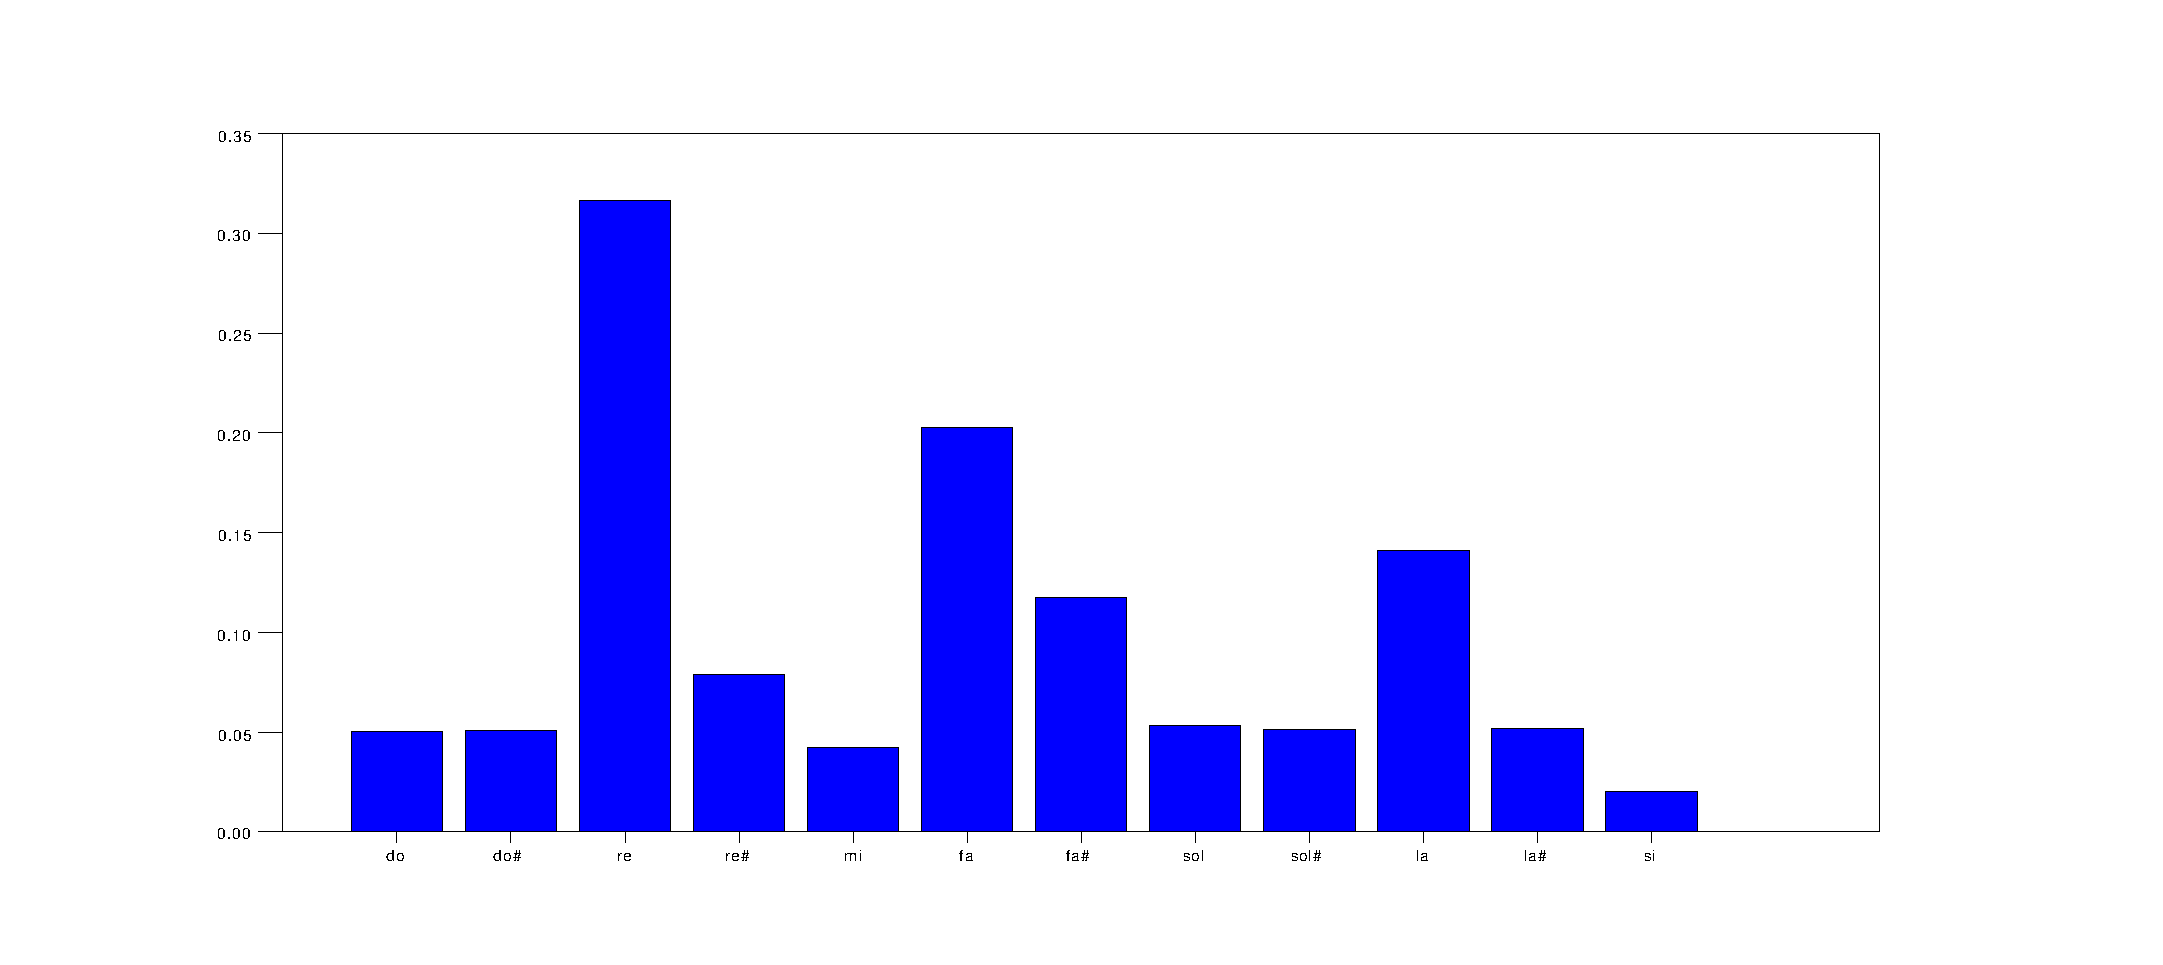
\includegraphics[keepaspectratio=true,scale=0.49]{figuras/Dm/notas_Dm.eps}
	\caption{Gráfico de sugestão de notas para a gravação do acorde $Dm$.}
  \label{fig:notas_Dm}
\end{figure}

\begin{figure}[h]
	\centering
		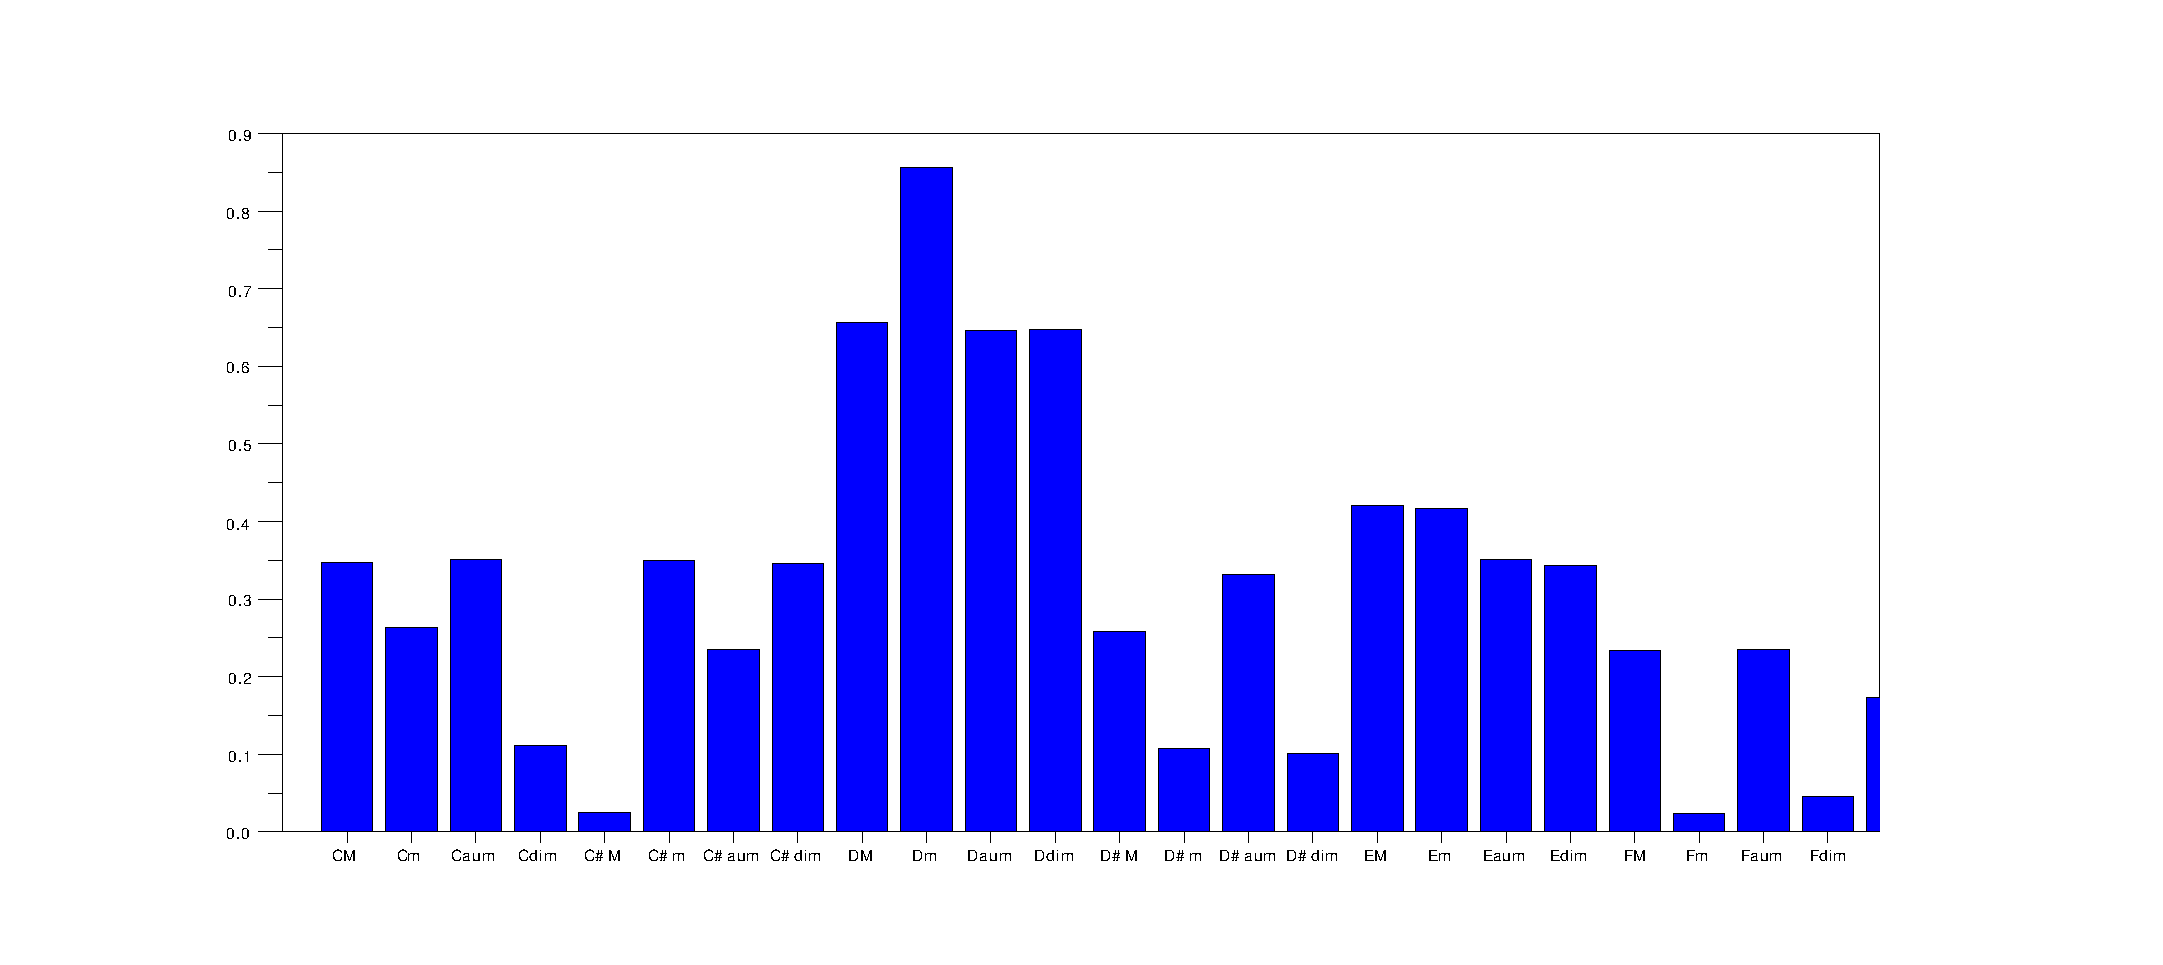
\includegraphics[keepaspectratio=true,scale=0.49]{figuras/Dm/acordes_1_Dm.eps}
		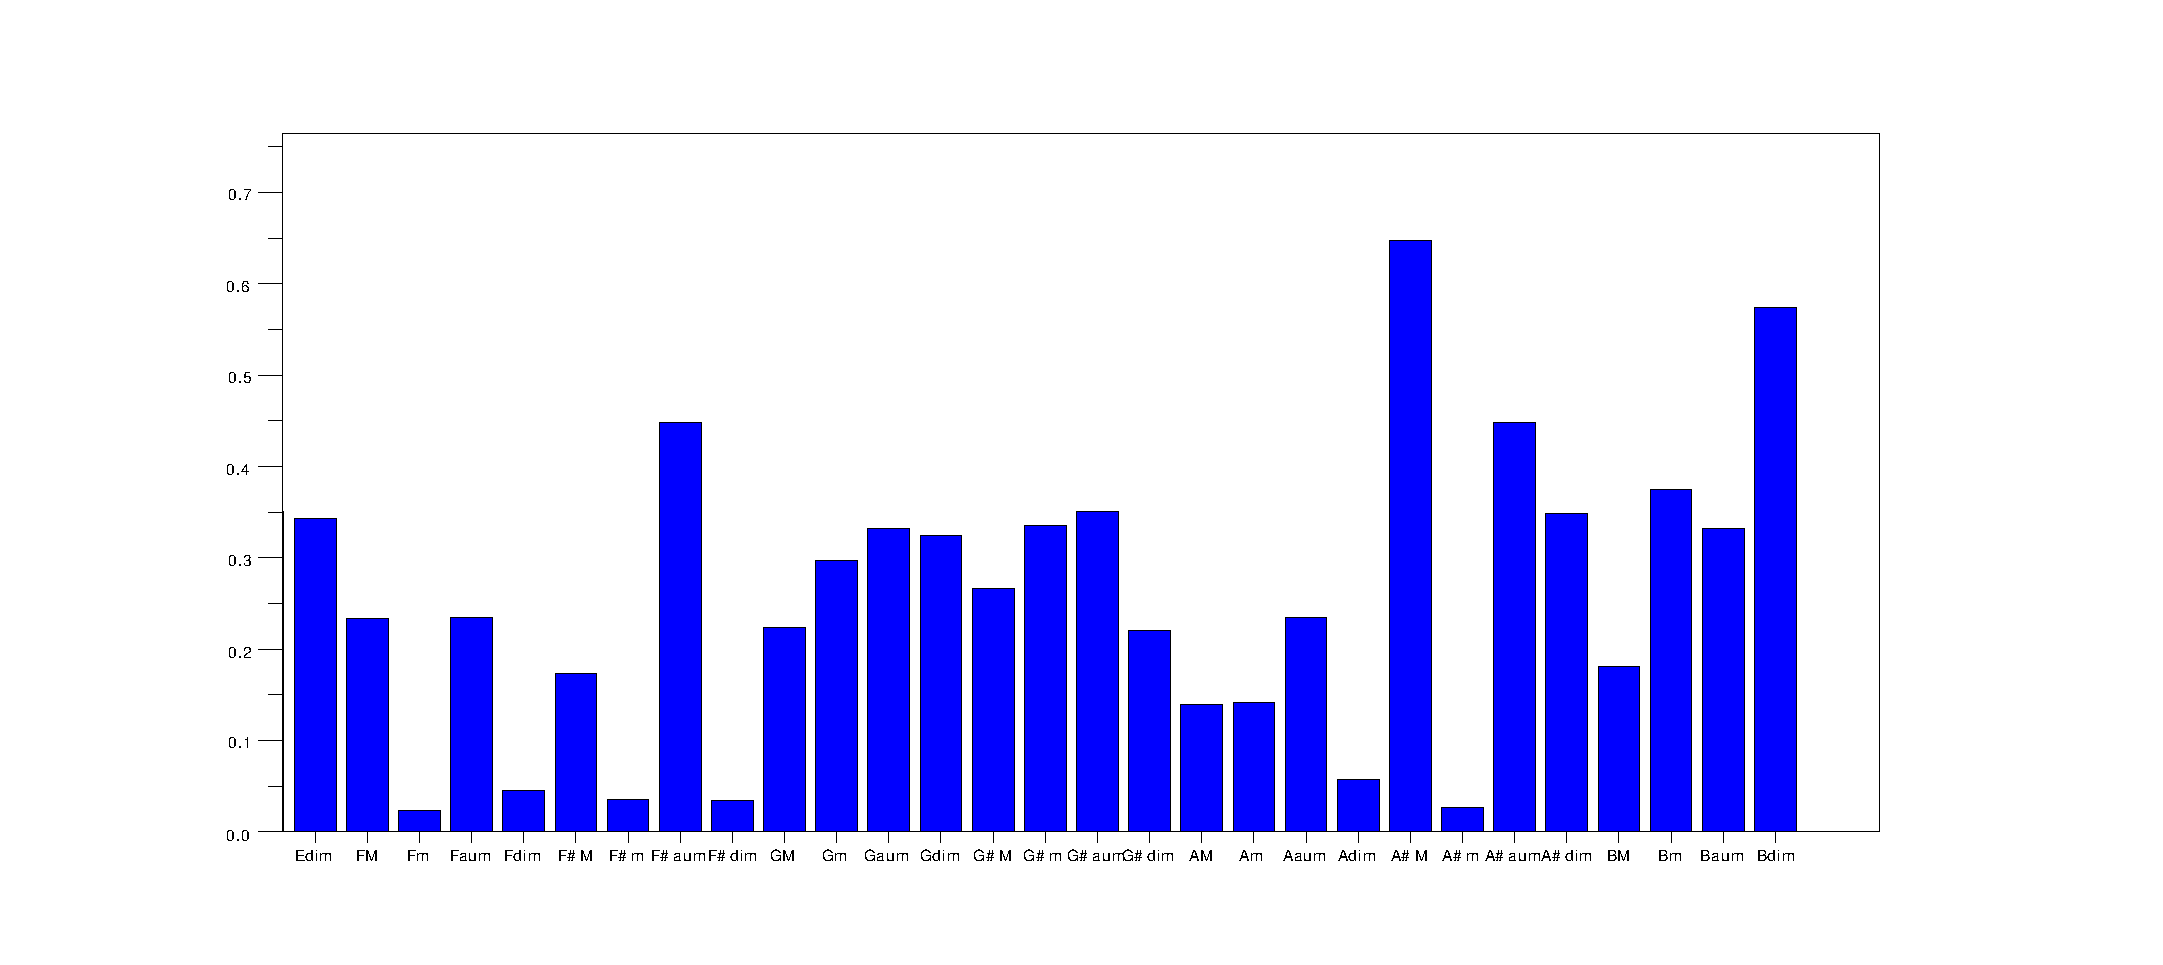
\includegraphics[keepaspectratio=true,scale=0.49]{figuras/Dm/acordes_2_Dm.eps}
	\caption{Gráficos de sugestão de acordes a gravação do acorde $Dm$.}
  \label{fig:acordes_Dm}
\end{figure}


Do resultado da primeira camada de processamento é gerado o gráfico da figura \ref{fig:espectro_Dm}. Esse gráfico diz respeito a natureza da composição do sinal em senoides em termos de transformada de fourier. O primeiro pico, no valor de 294 Hz, é relativo a nota $Ré$. O segundo pico, no valor de 350 Hz, é relativo a nota $Fá$. O terceiro pico, no valor de 441 Hz, é relativo a nota $Lá$. Os picos seguintes são relativos aos harmônicos dessas três notas.

Do resultado da segunda camada de processamento é gerado gráfico da figura \ref{fig:notas_Dm}. É possível perceber nele que as notas $Ré$, $Fá$ e $Lá$ são as que mais possuem energia ou, no ponto de vista de sugestão, as mais sugeridas. De certa forma um dos fatores que contribuiram das notas $Ré$ e $Lá$ ser de maiores energias foi devido a presença dos harmônicos.

Do resultado da terceira camada de processamento são gerados os gráficos da figura \ref{fig:acordes_Dm}. Essa camada é relativa ao resultados das sugestões de acordes musicais. É perceptível ver a presença da alta sugestão do acorde $Dm$.

\subsection{Experimento 3 - Acorde $Ddim$}
\label{sec:experimento3}

Nesse experimento foi tocado a tríade $Ré$ (baixo e tônica), $Fá$ e $Sol\#$ equivalente ao acorde Ddim. A tríade foi tocada ao mesmo tempo e com a mesma força para todas as notas.

Segue os gráficos resultantes:

\begin{figure}[h]
	\centering
		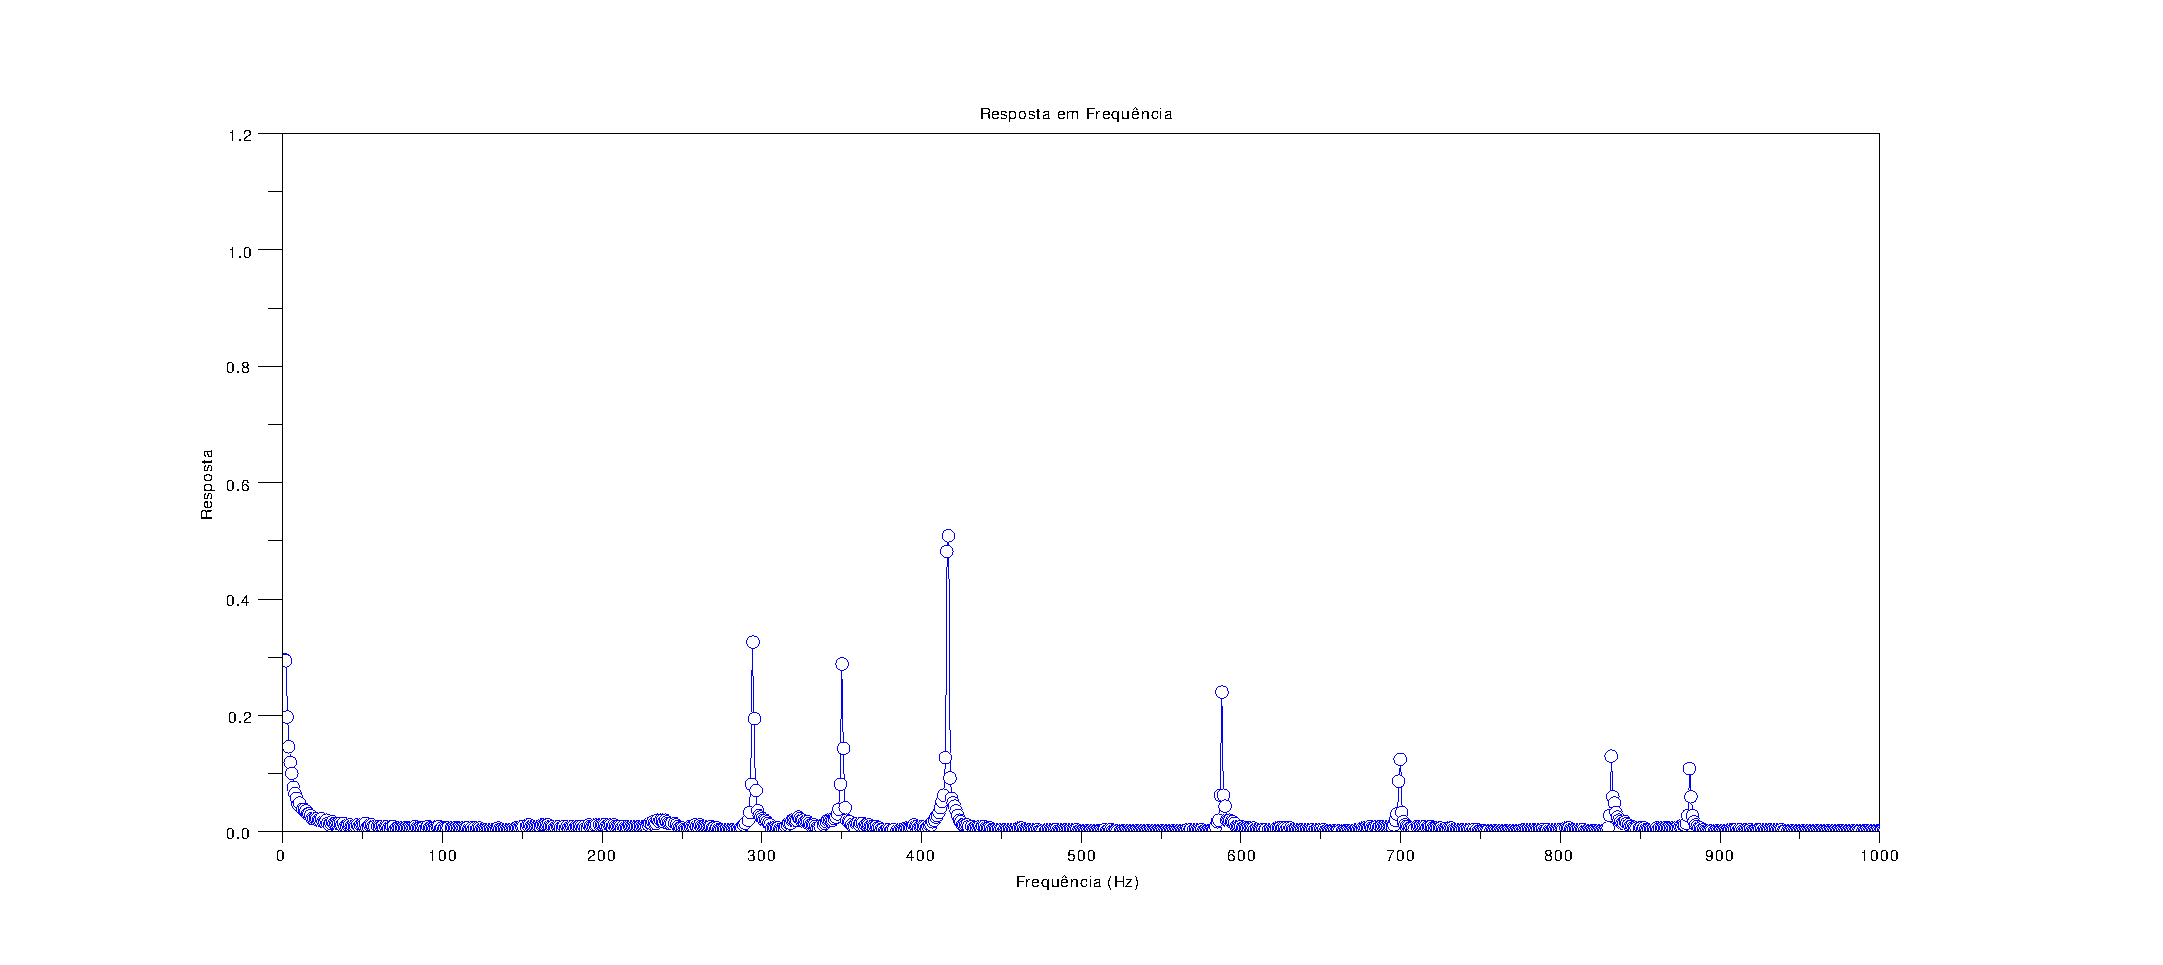
\includegraphics[keepaspectratio=true,scale=0.49]{figuras/Dm/fft_Ddim.eps}
	\caption{Gráfico da resposta em frequência para a gravação do acorde $Ddim$.}
  \label{fig:espectro_Ddim}
\end{figure}

\begin{figure}[h]
	\centering
		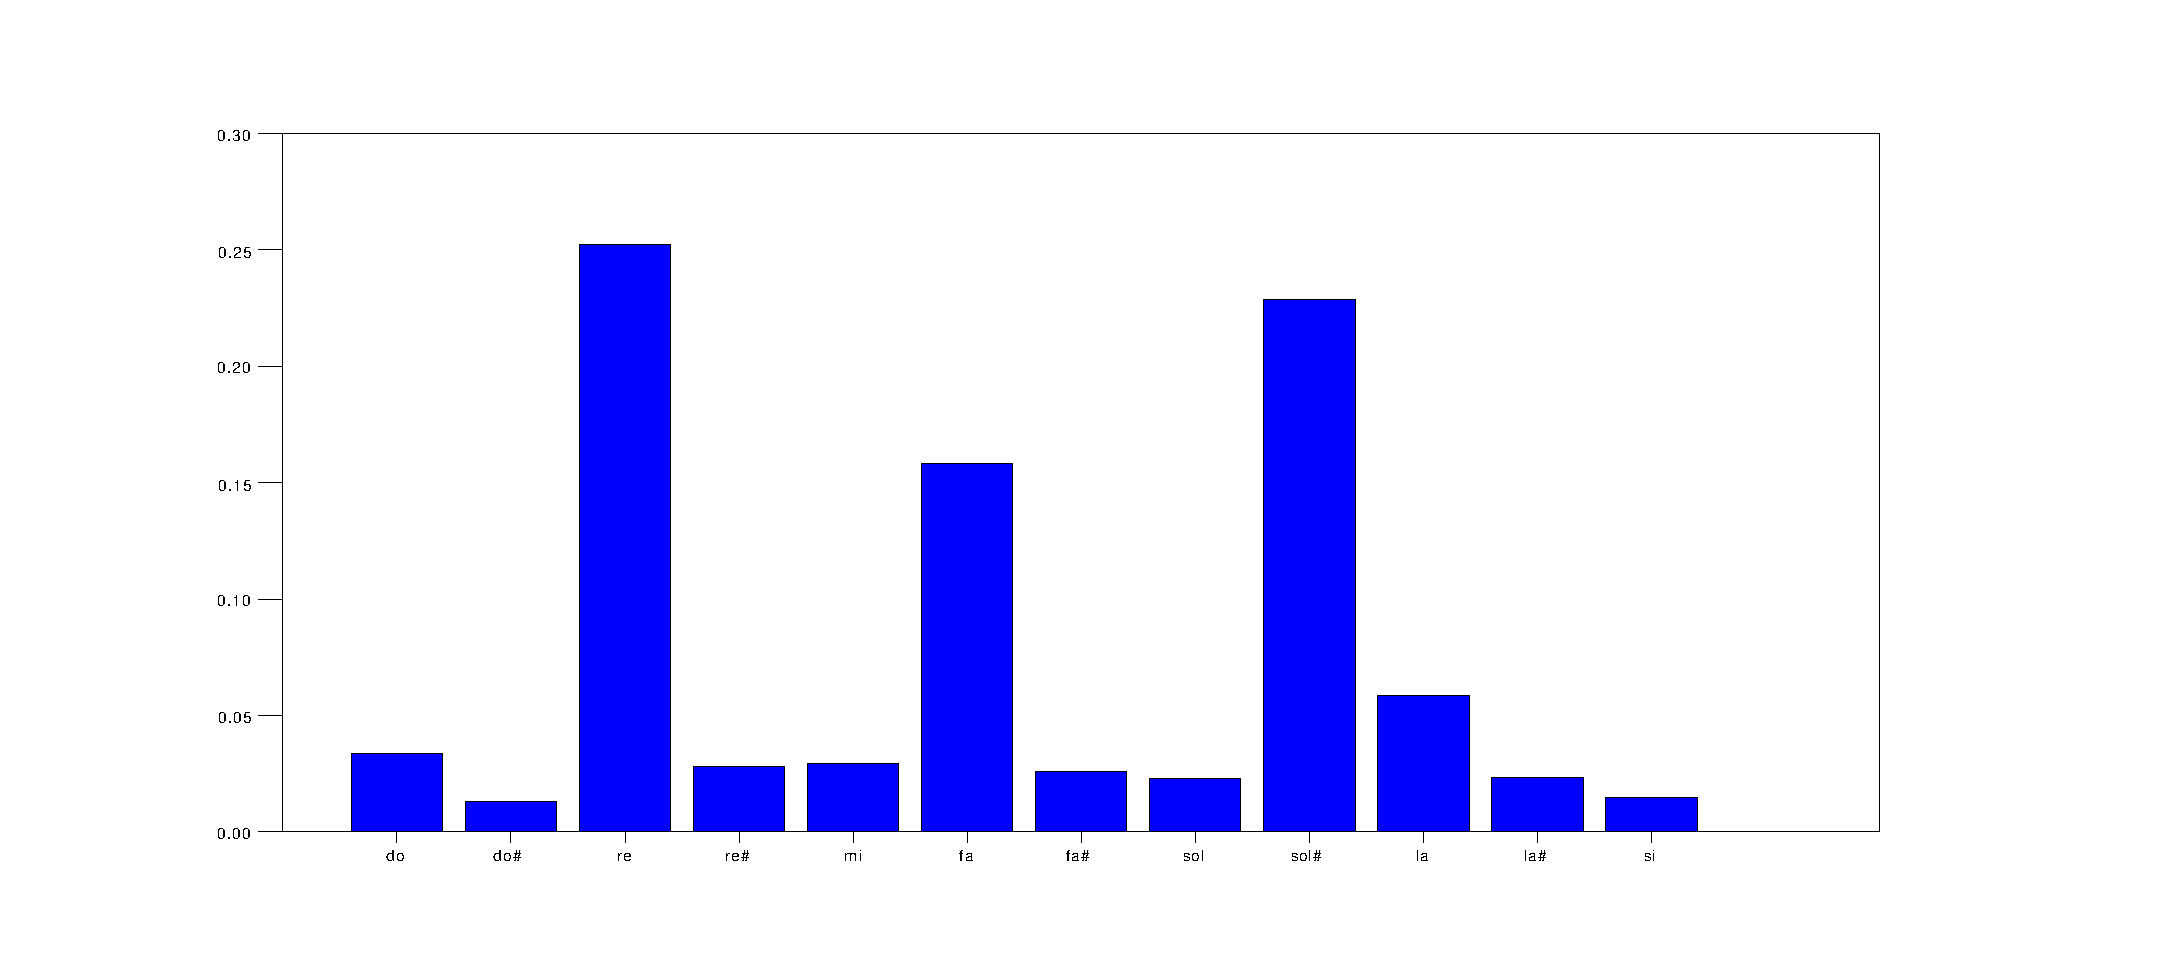
\includegraphics[keepaspectratio=true,scale=0.45]{figuras/Dm/notas_Ddim.eps}
	\caption{Gráfico de sugestão de notas para a gravação do acorde $Ddim$.}
  \label{fig:notas_Ddim}
\end{figure}

\begin{figure}[h]
	\centering
		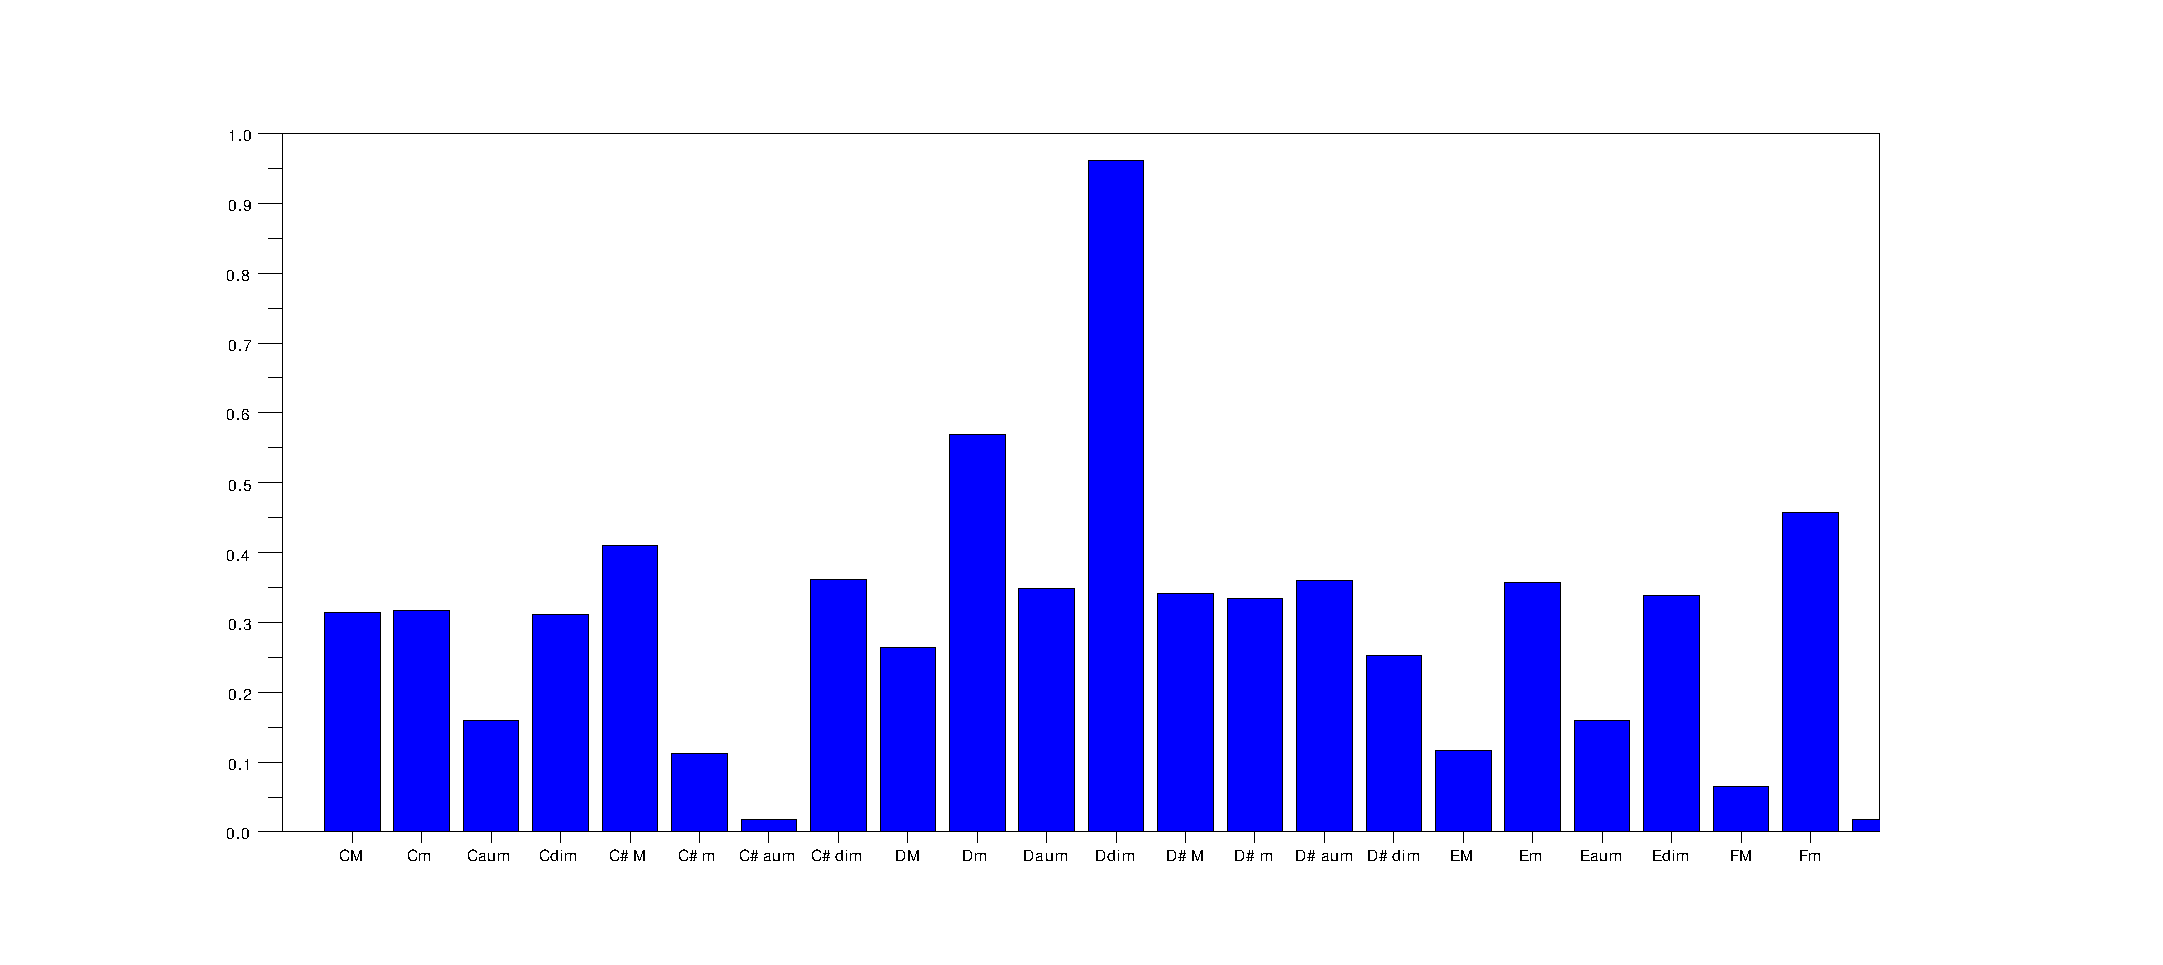
\includegraphics[keepaspectratio=true,scale=0.49]{figuras/Dm/acordes_1_Ddim.eps}
		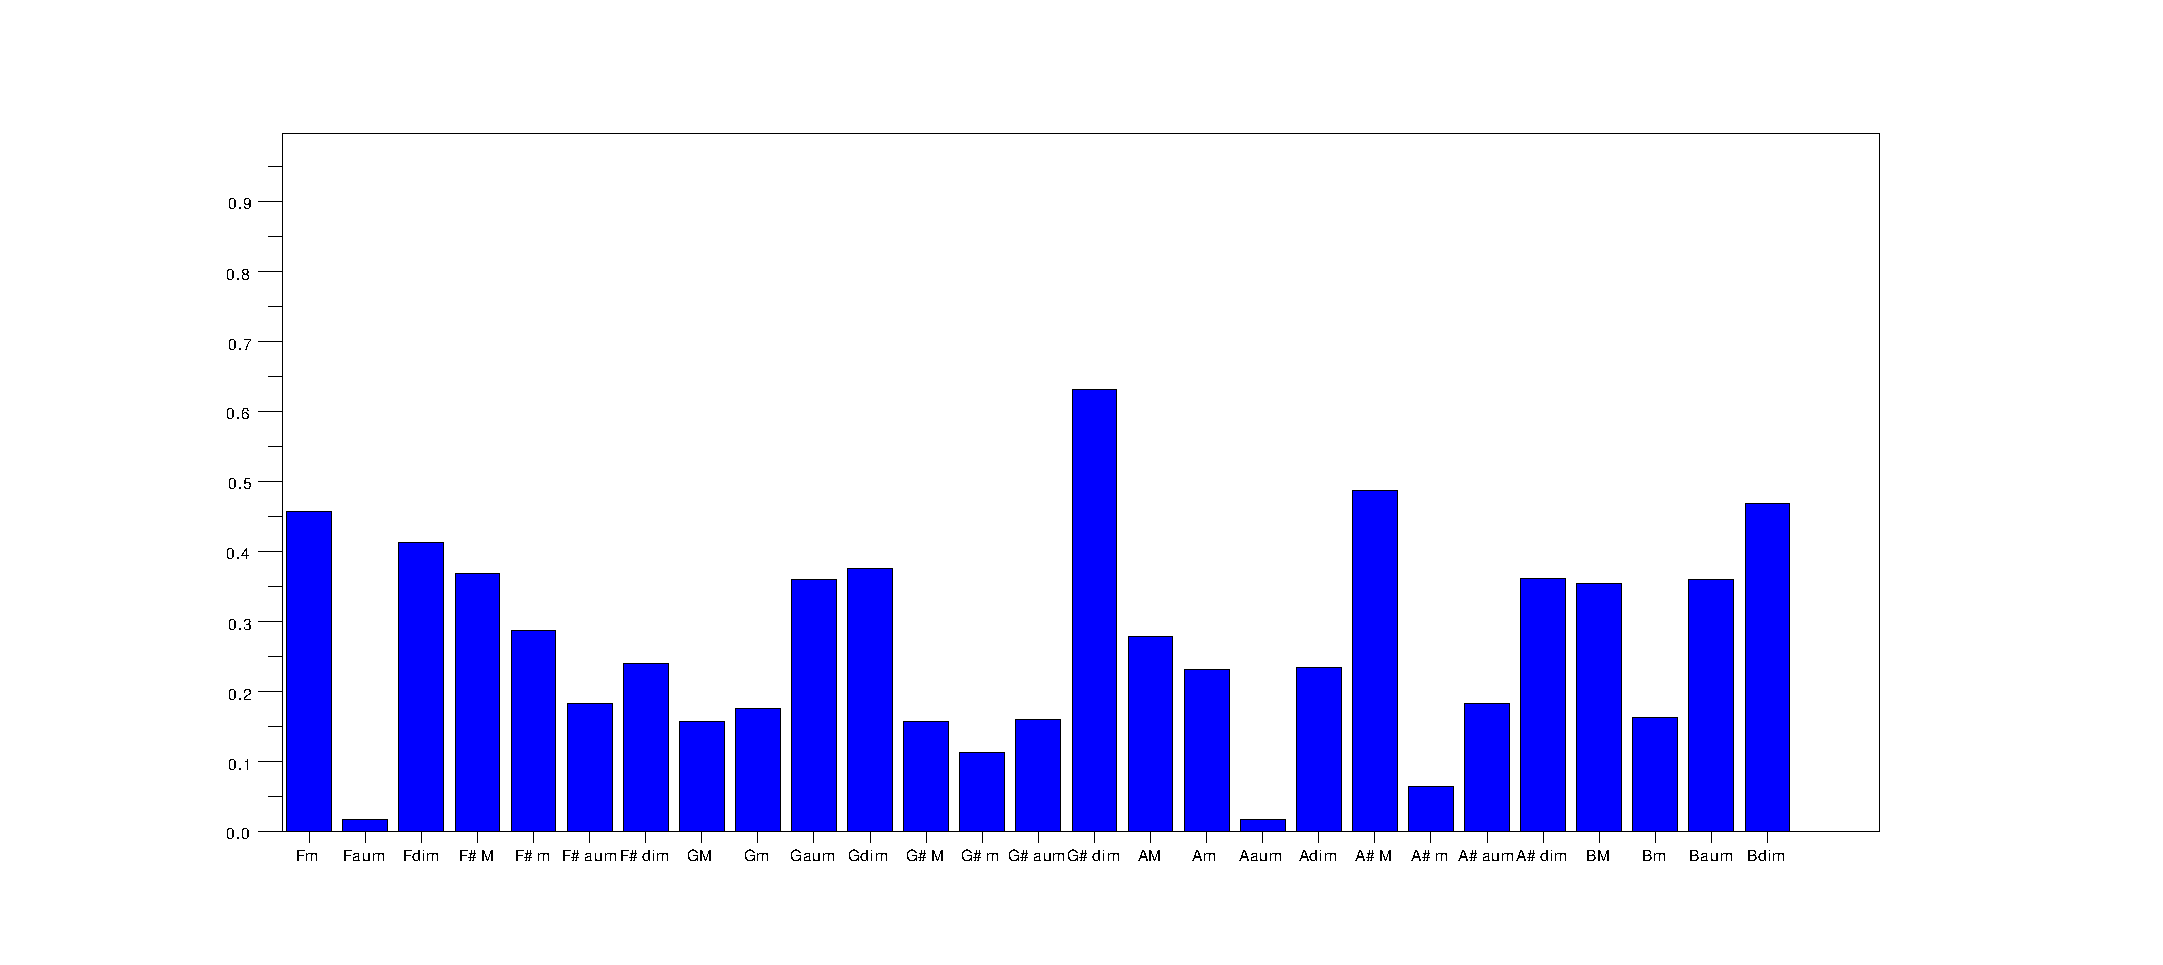
\includegraphics[keepaspectratio=true,scale=0.49]{figuras/Dm/acordes_2_Ddim.eps}
	\caption{Gráficos de sugestão de acordes a gravação do acorde $Ddim$.}
  \label{fig:acordes_Ddim}
\end{figure}


Do resultado da primeira camada de processamento é gerado o gráfico da figura \ref{fig:espectro_Ddim}. Esse gráfico diz respeito a natureza da composição do sinal em senoides em termos de transformada de fourier. O primeiro pico, no valor de 294 Hz, é relativo a nota $Ré$. O segundo pico, no valor de 350 Hz, é relativo a nota $Fá$. O terceiro pico, no valor de 417 Hz, é relativo a nota $Sol\#$. Os picos seguintes são relativos aos harmônicos dessas três notas.

Do resultado da segunda camada de processamento é gerado gráfico da figura \ref{fig:notas_Ddim}. É possível perceber nele que as notas $Ré$, $Fá$ e $Sol\#$ são as que mais possuem energia ou, no ponto de vista de sugestão, as mais sugeridas.

Do resultado da terceira camada de processamento são gerados os gráficos da figura \ref{fig:acordes_Ddim}. Essa camada é relativa ao resultados das sugestões de acordes musicais. É perceptível ver a presença da alta sugestão do acorde $Ddim$.

\subsection{Experimento 4 - Acorde $Daum$}
\label{sec:experimento4}

Nesse experimento foi tocado a tríade $Ré$ (baixo e tônica), $Fá\#$ e $Lá\#$ equivalente ao acorde $Daum$. A tríade foi tocada ao mesmo tempo e com a mesma força para todas as notas.

Segue os gráficos resultantes:

\begin{figure}[h]
	\centering
		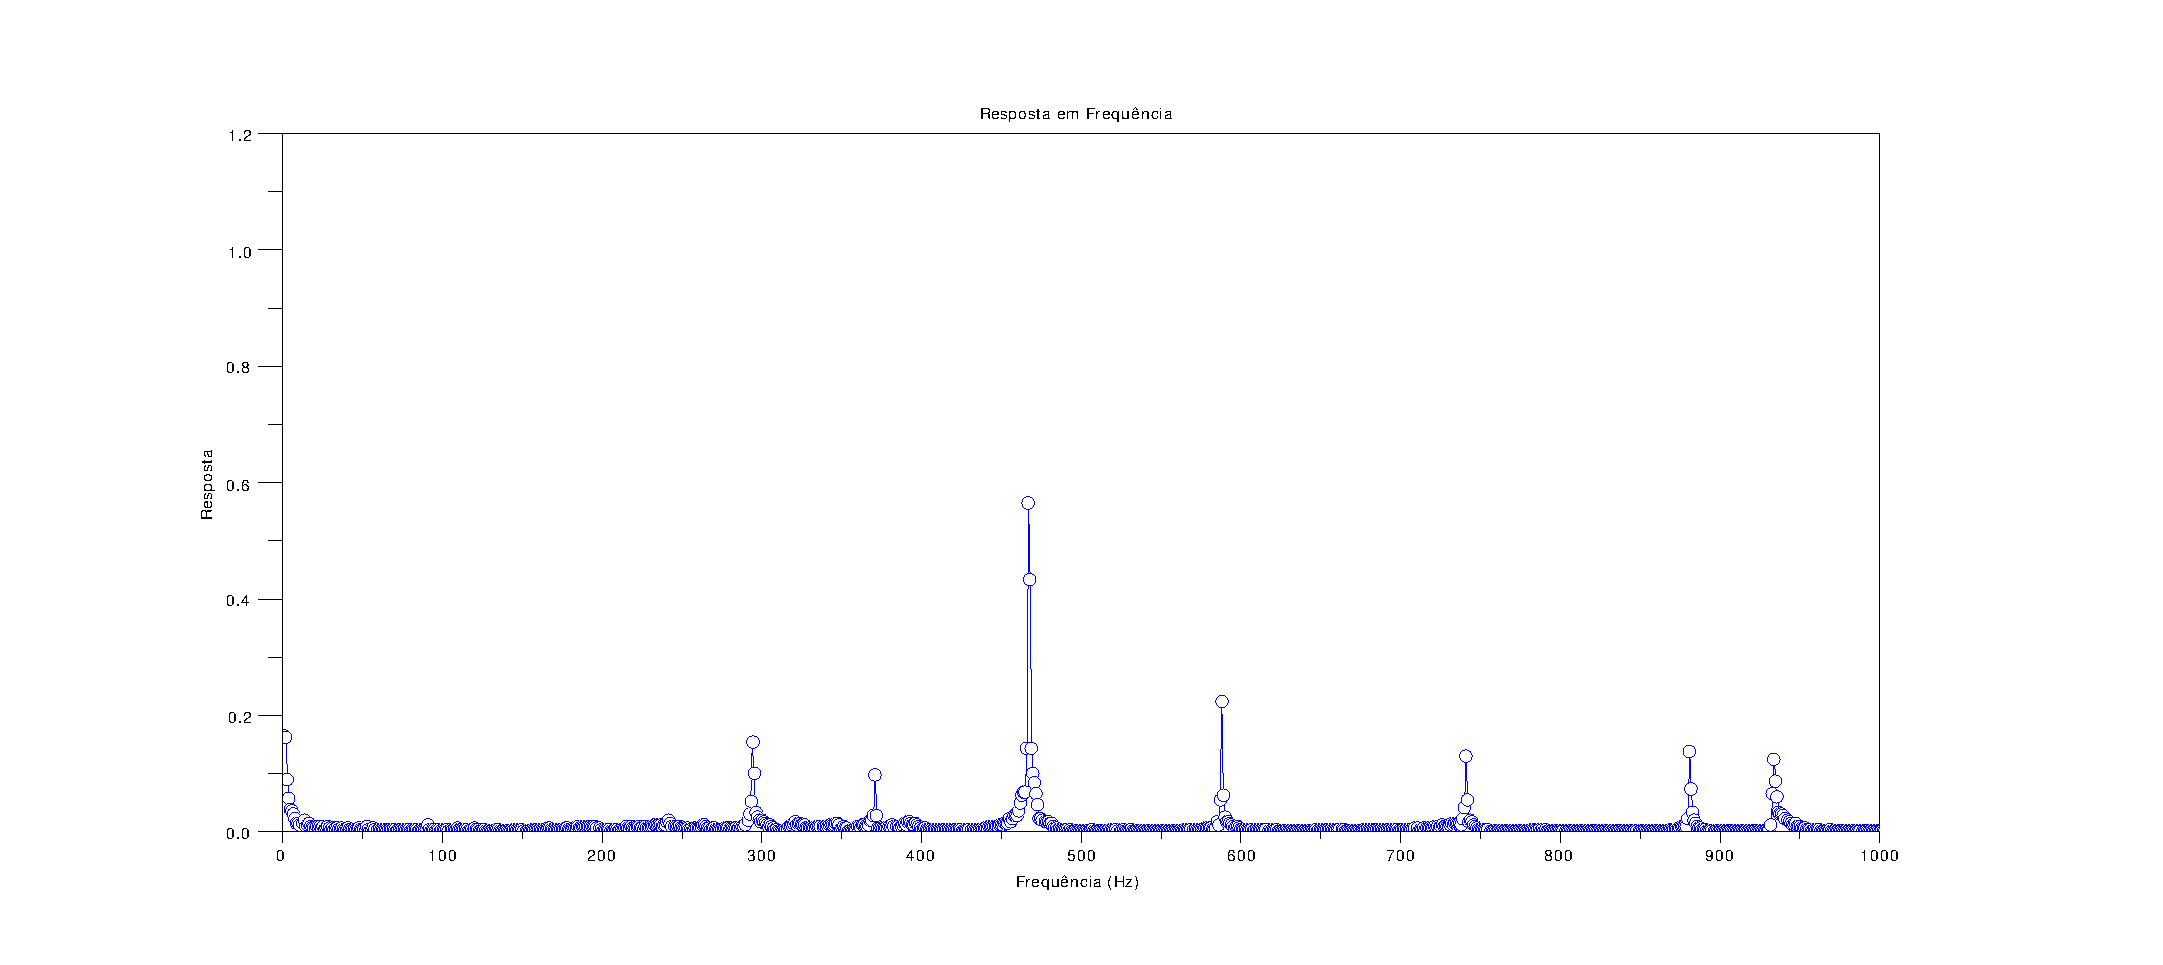
\includegraphics[keepaspectratio=true,scale=0.49]{figuras/Dm/fft_Daum.eps}
	\caption{Gráfico da resposta em frequência para a gravação do acorde $Daum$.}
  \label{fig:espectro_Daum}
\end{figure}

\begin{figure}[h]
	\centering
		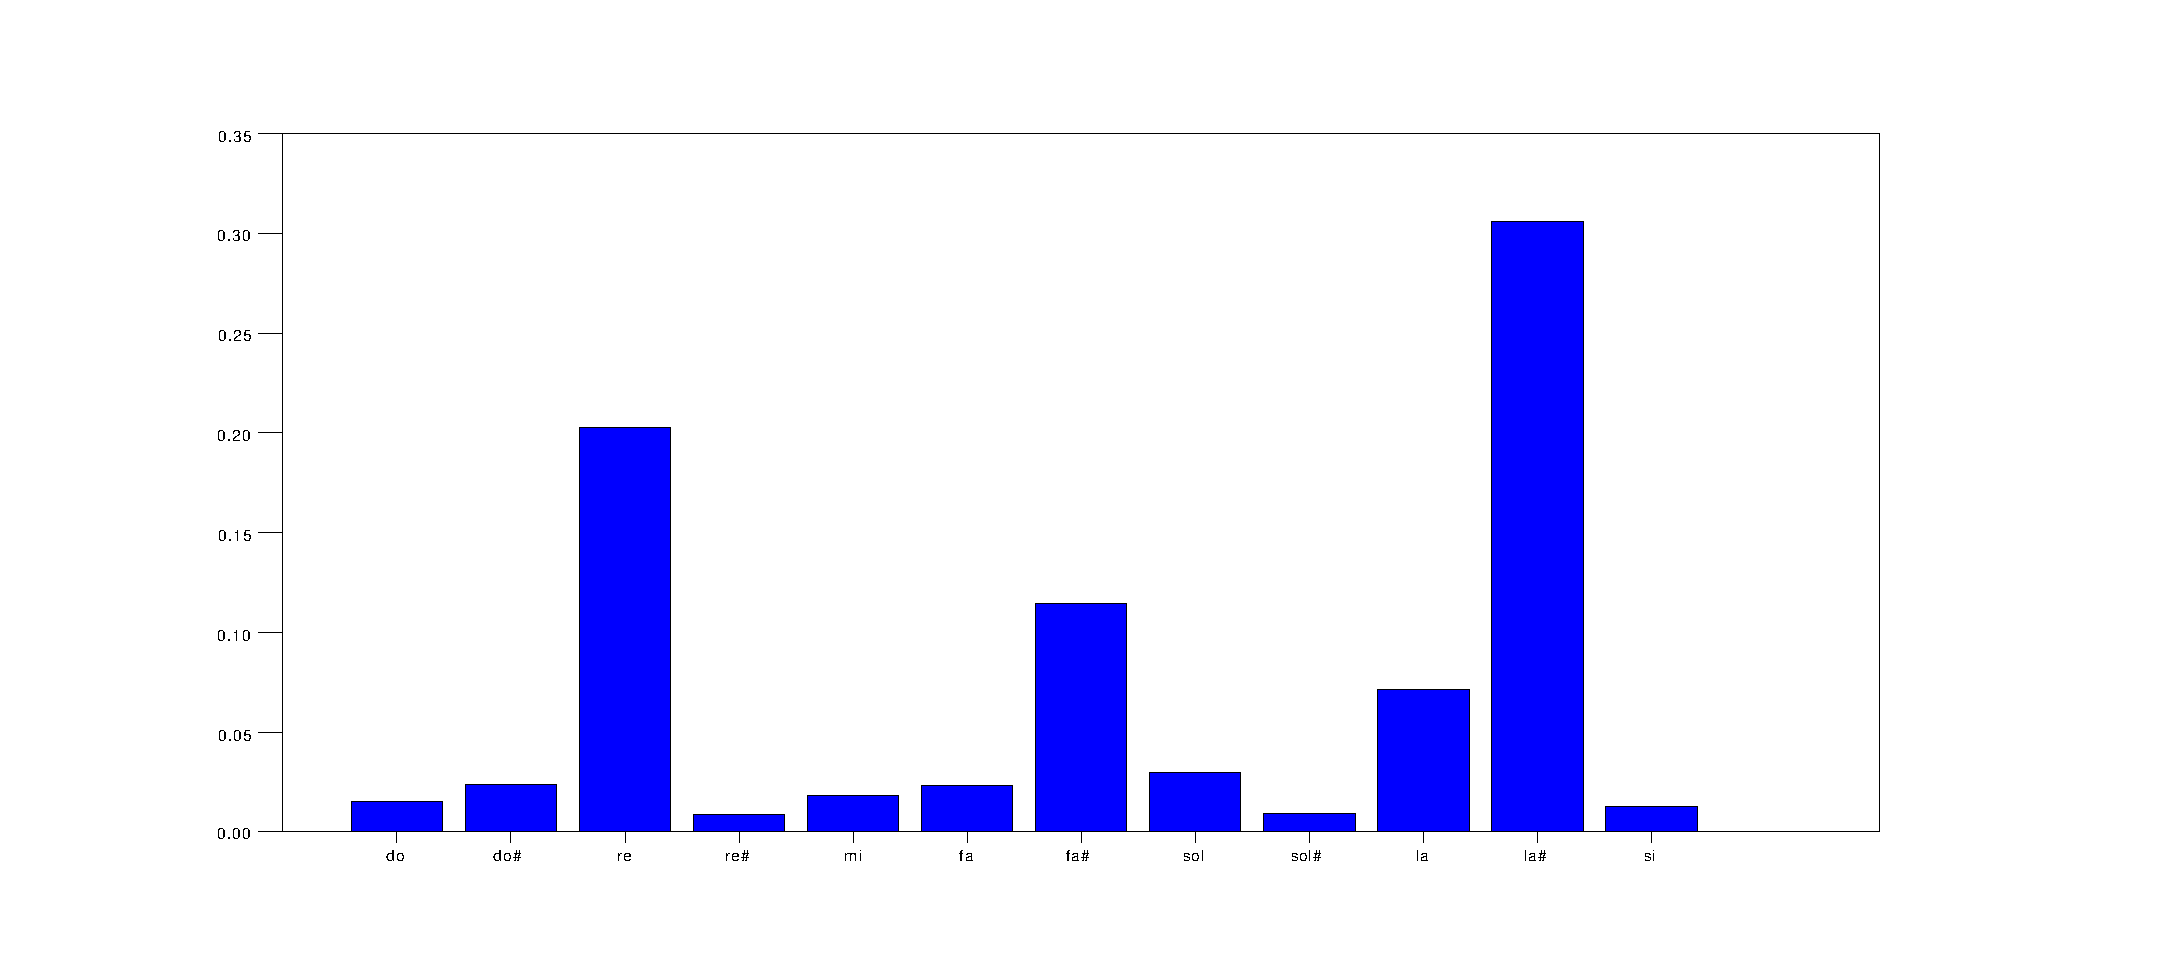
\includegraphics[keepaspectratio=true,scale=0.49]{figuras/Dm/notas_Daum.eps}
	\caption{Gráfico de sugestão de notas para a gravação do acorde $Daum$.}
  \label{fig:notas_Daum}
\end{figure}

\begin{figure}[h]
	\centering
		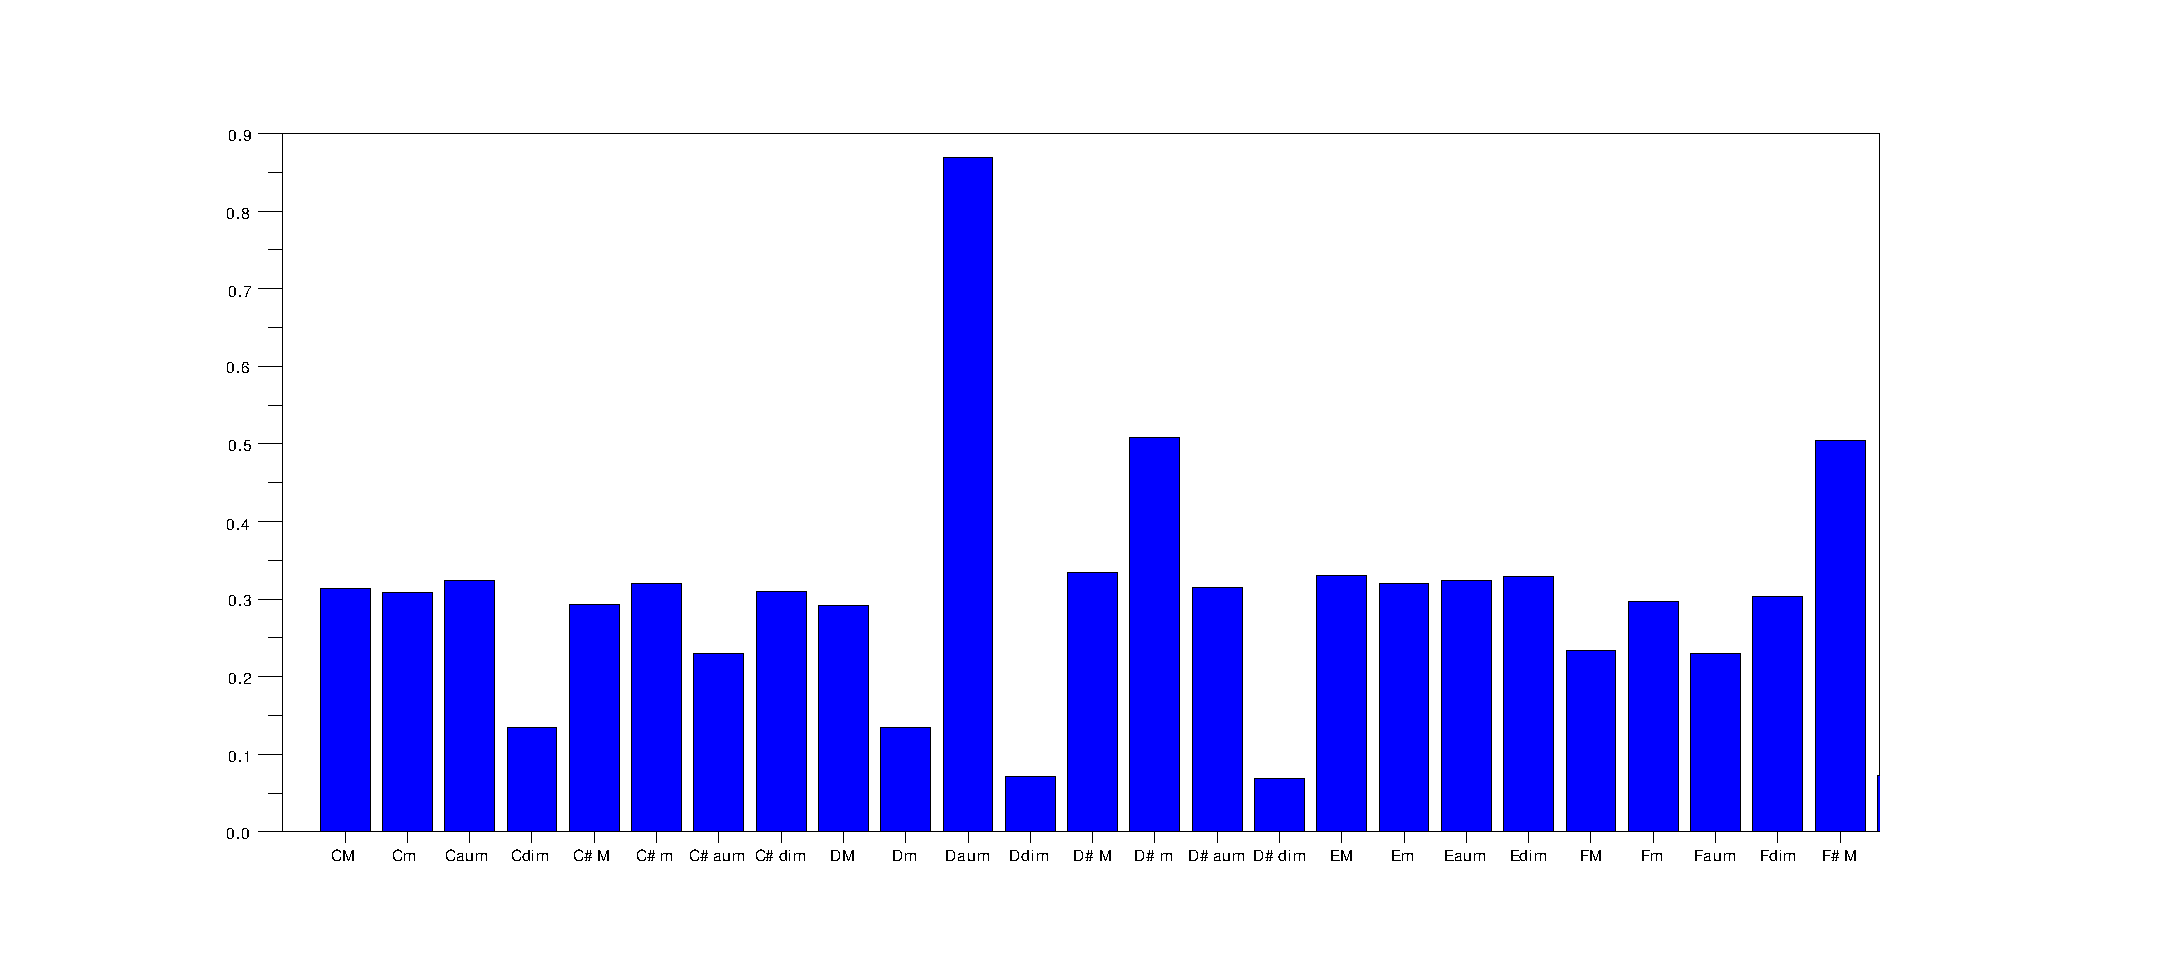
\includegraphics[keepaspectratio=true,scale=0.49]{figuras/Dm/acordes_1_Daum.eps}
		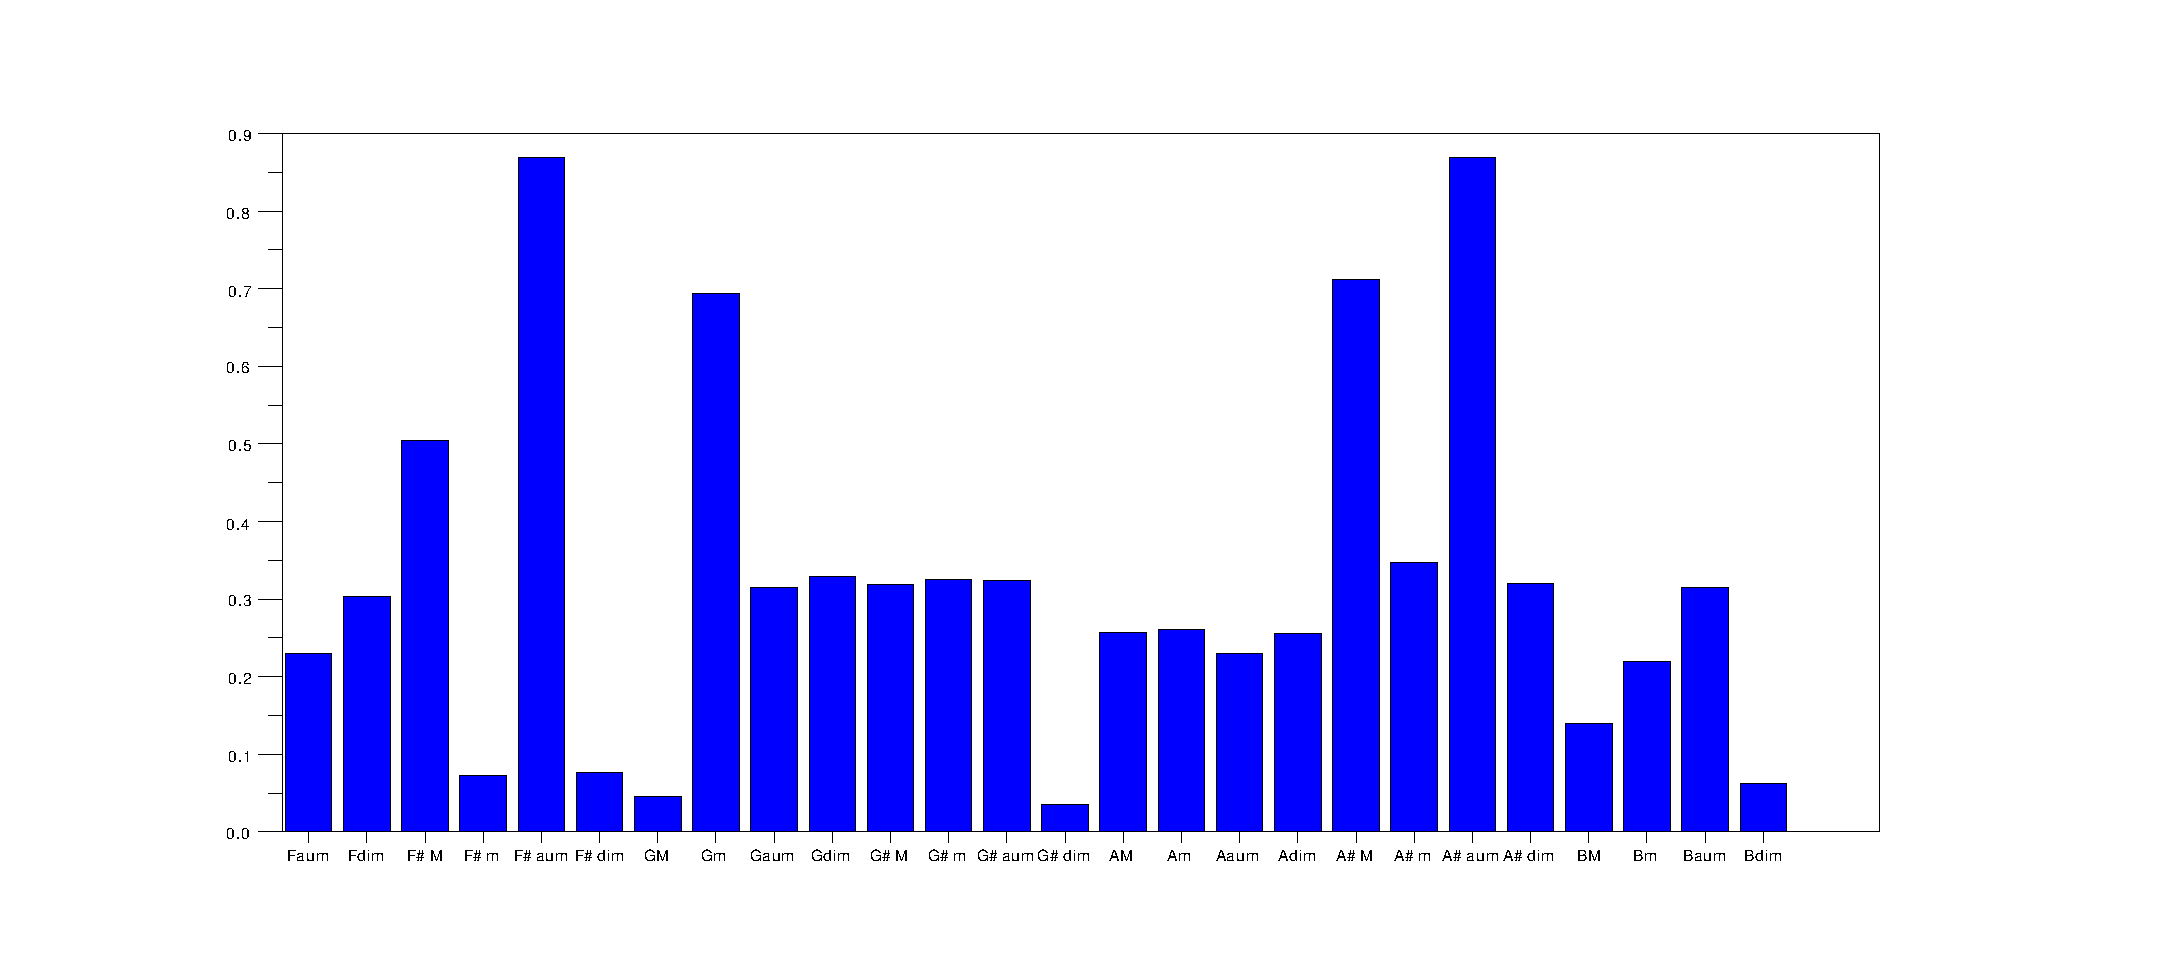
\includegraphics[keepaspectratio=true,scale=0.49]{figuras/Dm/acordes_2_Daum.eps}
	\caption{Gráficos de sugestão de acordes a gravação do acorde $Daum$.}
  \label{fig:acordes_Daum}
\end{figure}


Do resultado da primeira camada de processamento é gerado o gráfico da figura \ref{fig:espectro_Daum}. Esse gráfico diz respeito a natureza da composição do sinal em senoides em termos de transformada de fourier. O primeiro pico, no valor de 294 Hz, é relativo a nota $Ré$. O segundo pico, no valor de 371 Hz, é relativo a nota $Fá\#$. O terceiro pico, no valor de 467 Hz, é relativo a nota $Lá\#$. Os picos seguintes são relativos aos harmônicos dessas três notas.

Do resultado da segunda camada de processamento é gerado gráfico da figura \ref{fig:notas_Daum}. É possível perceber nele que as notas $Ré$, $Fá\#$ e $Lá\#$ são as que mais possuem energia ou, no ponto de vista de sugestão, as mais sugeridas.

Do resultado da terceira camada de processamento são gerados os gráficos da figura \ref{fig:acordes_Daum}. Essa camada é relativa aos resultados das sugestões de acordes musicais. É perceptível a alta sugestão dos acordes $Daum$, $F\#aum$ e $A\#aum$ com a mesma quantidade de energia. Isso é devido às notas comporem os mesmos acordes, diferenciando um do outro somente pela nota mais grave da tríade. Visto que o sistema possui o módulo de extração de baixos, a solução indicou que o acorde tocado foi $Daum$, visto que, como é mostrado no gráfico do espectro de frequências, a nota $Ré$ é a nota mais grave da tríade.

A tabela \ref{tab:label_test} mostra os resultados do sistema dado todas as combinações dos conjuntos de acordes de tríades possíveis. Esses resultados foram gerados pelo script disponível no repositório desse trabalho \footnote{https://github.com/josepedro/TCC}.

\begin{table}[h]
  %Vertical lines as column separators
  \centering
  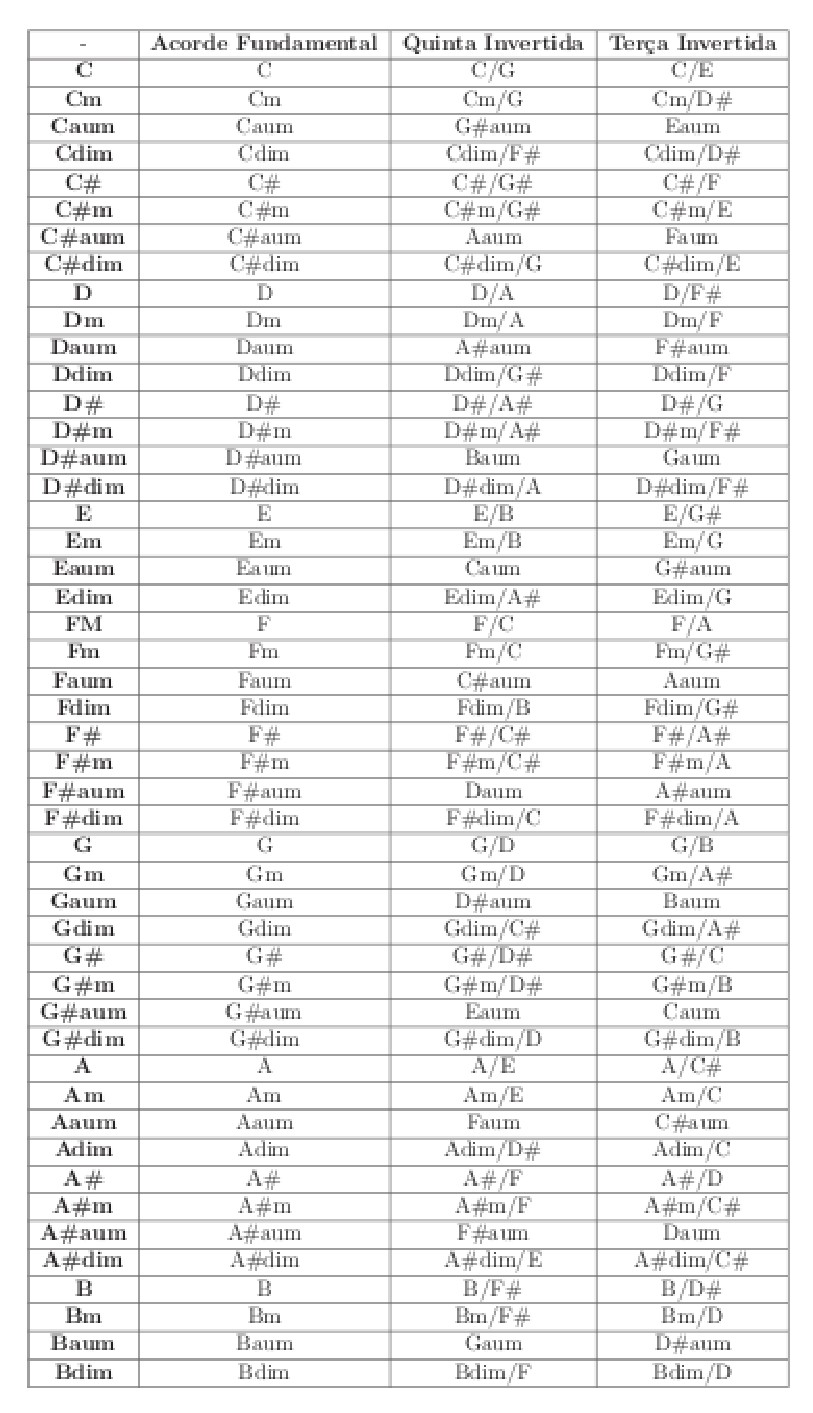
\includegraphics[keepaspectratio=true,scale=0.8]{figuras/tabela_acordes_completos.eps}
  \caption{Tabela de resultados dado os acordes tocados com inversões.}
  \label{tab:label_test}
\end{table}

\section{Detecção de Transições Rítmicas}

Com o intuito de detectar acordes ao longo do tempo, foi pensado um algoritmo baseado em correlação de níveis de energia ao longo do tempo abordado no ciclo de desenvolvimento \ref{subsec:ciclo_5} que delimitaria, em teoria, número de ocorrências e instante de ocorrência de acordes. Com essa delimitação seria possível ajustar a janela de análise em frequência nos limites energéticos. A figura \ref{fig:deteccao_ritmica_1} ilustra um exemplo de acordes tocados ao longo do tempo. 

\begin{figure}[h]
    \centering
    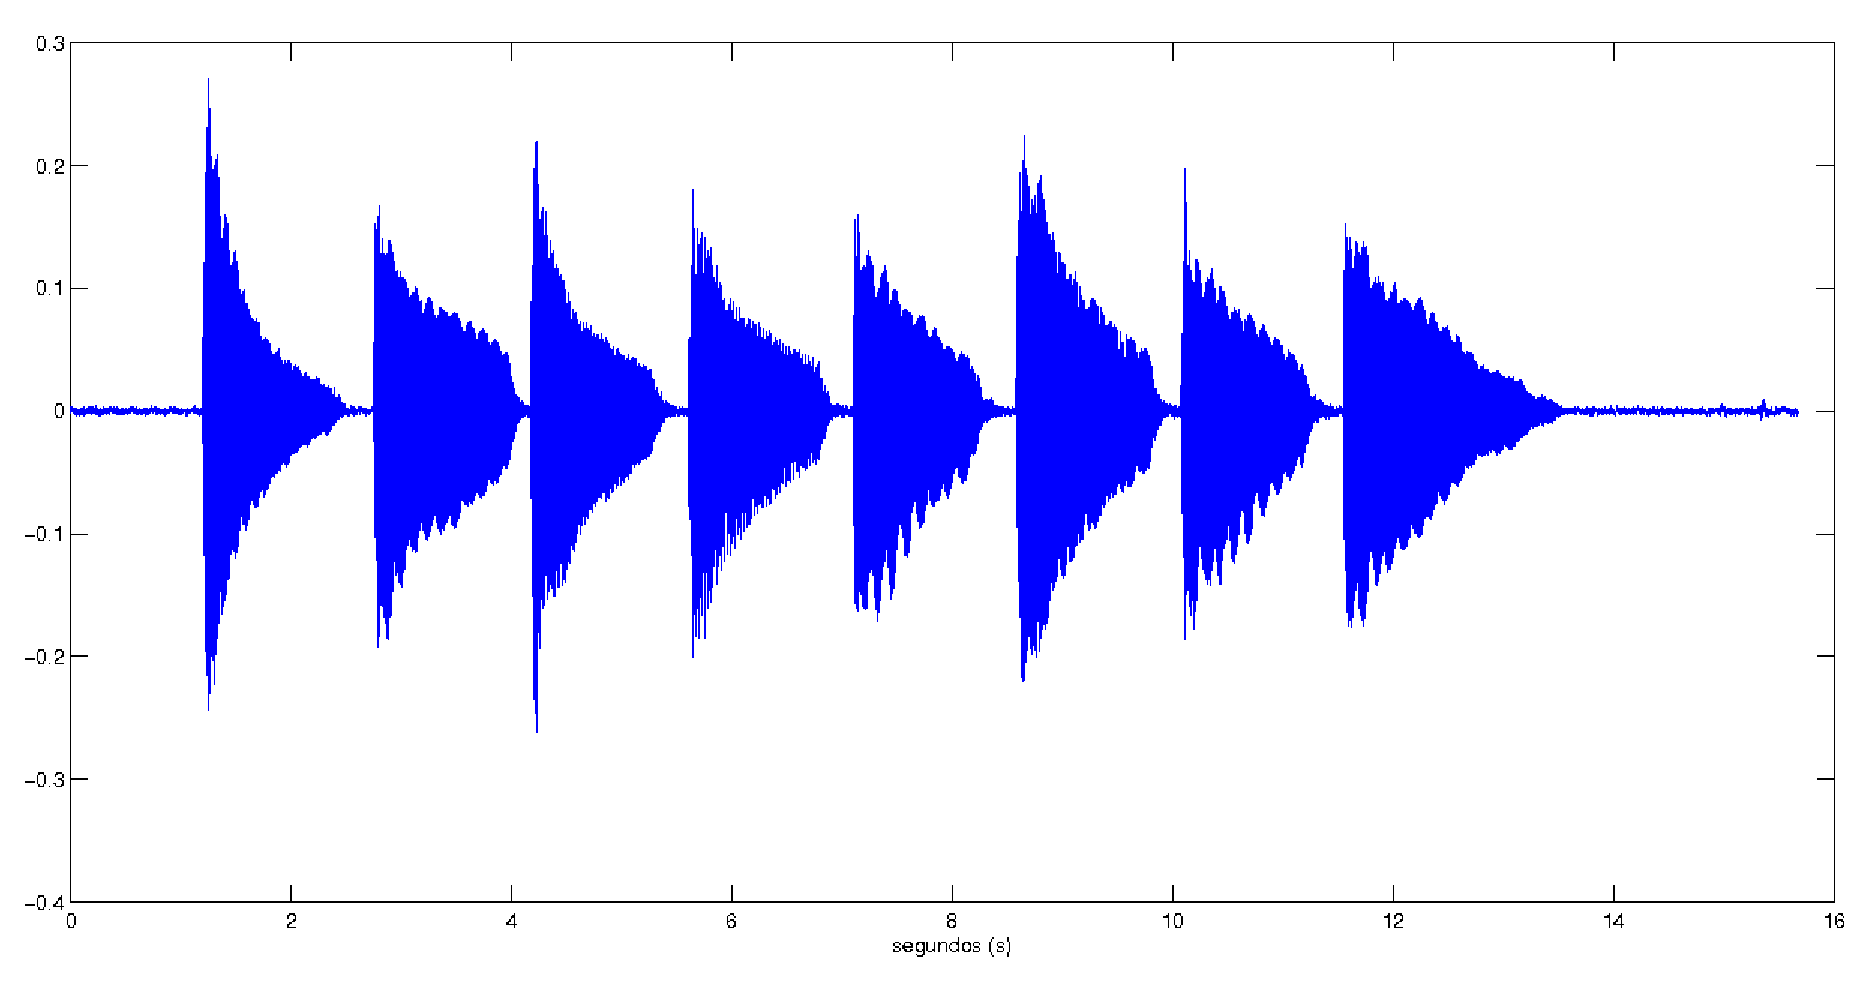
\includegraphics[keepaspectratio=true,scale=0.45]{figuras/deteccao_ritmica_1.eps}
  \caption{Acordes tocados ao longo do tempo.}
  \label{fig:deteccao_ritmica_1}
\end{figure}

Na figura acima é perceptível observar, pelos níveis de energia, 8 acordes tocados. Para validar a solução, o gráfico de picos de transição rítmica deverá apresentar 8 picos ao longo do tempo, destacando, além do número de picos, a localidade coesa de cada pico. A figura \ref{fig:deteccao_ritmica_2} mostra o gráfico de picos de transição rítmica.

\begin{figure}[h]
    \centering
    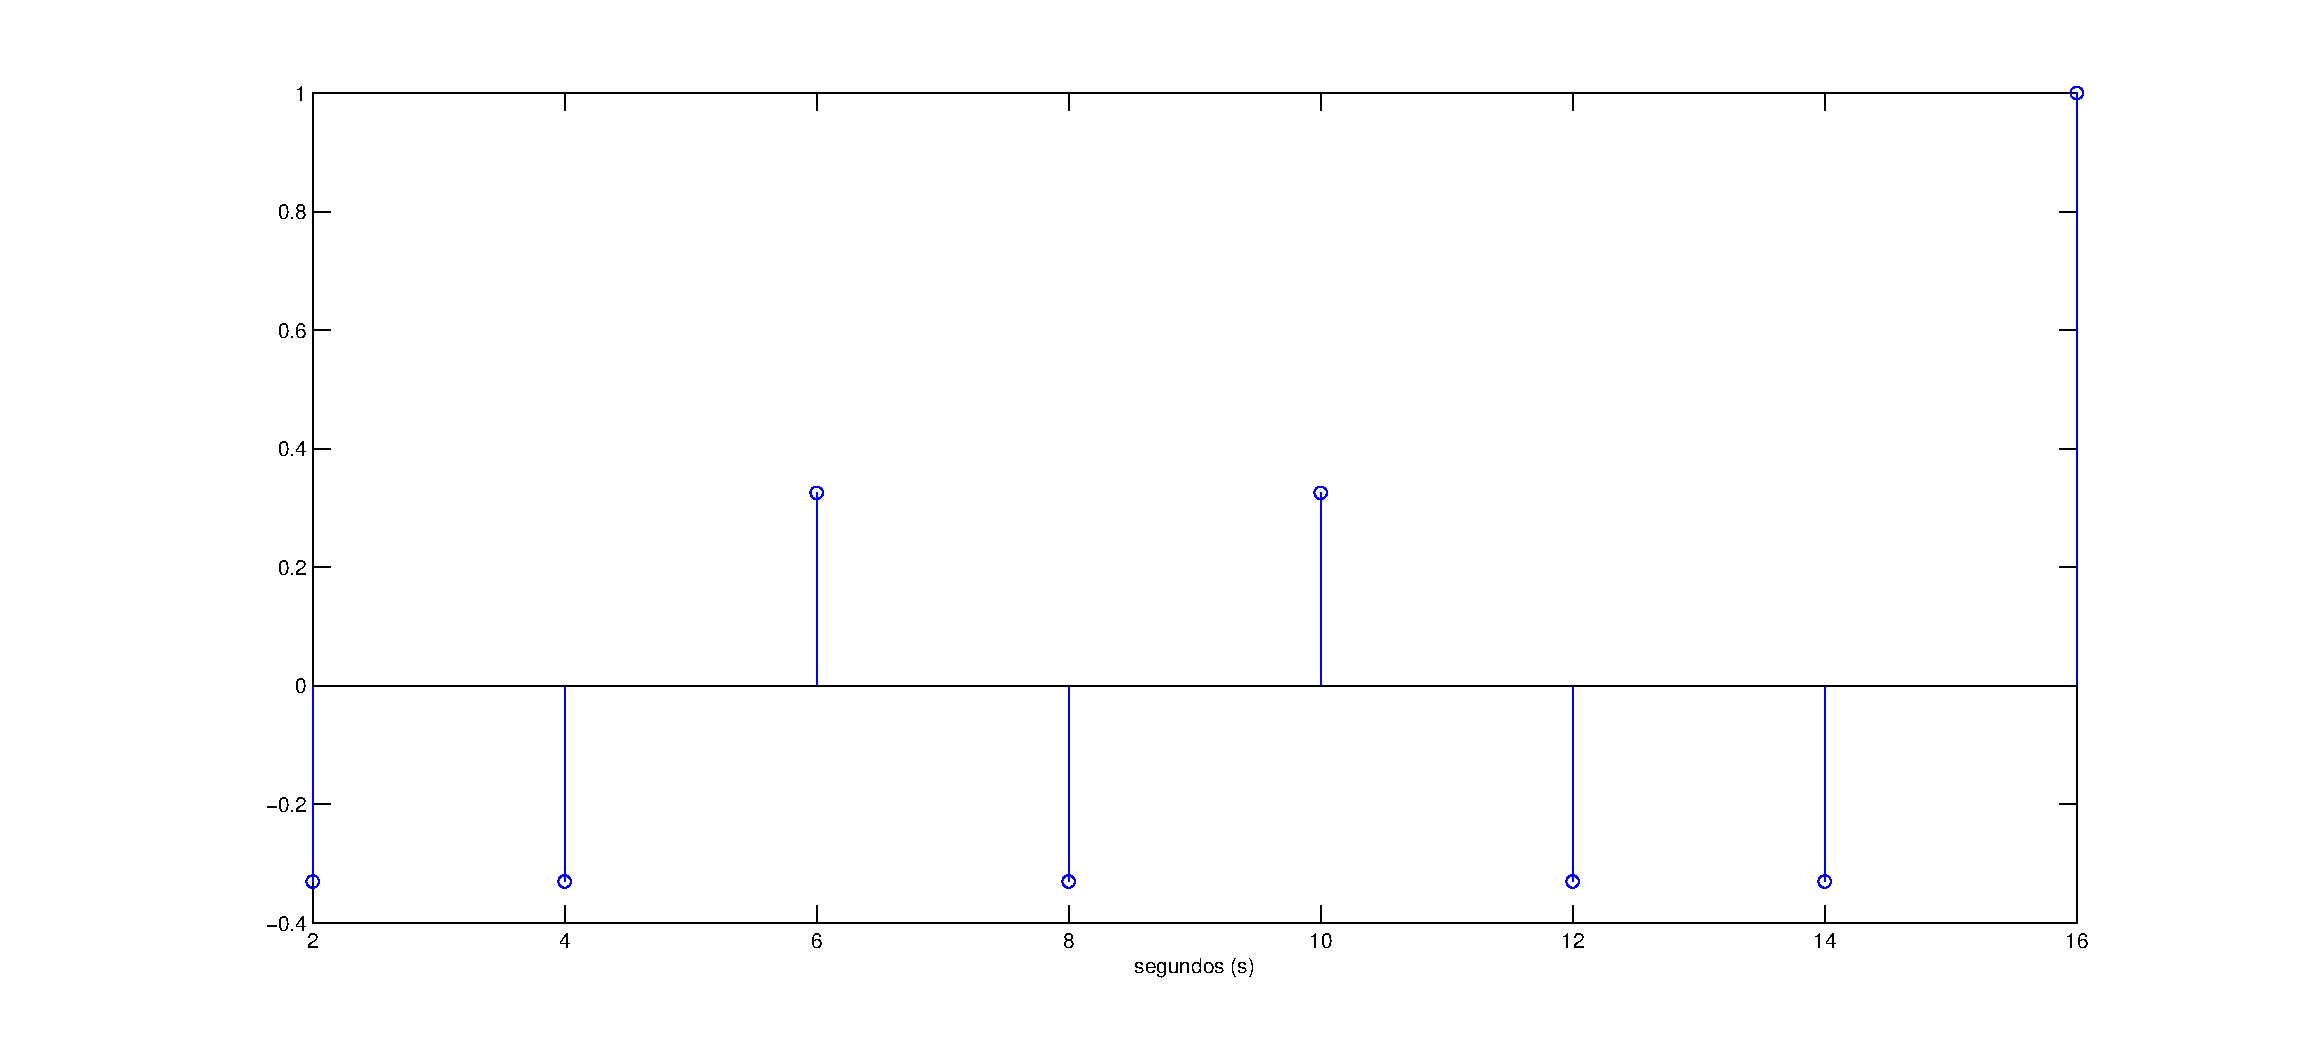
\includegraphics[keepaspectratio=true,scale=0.45]{figuras/deteccao_ritmica_2.eps}
  \caption{Gráfico de picos de transição rítmica.}
  \label{fig:deteccao_ritmica_2}
\end{figure}

Pode-se observar da figura acima que a quantidade de picos é coerente com a quantidade encontrada na figura \ref{fig:deteccao_ritmica_1}, entretanto os instantes das localidades dos picos não estão coerentes. Um exemplo desse fato é o último acorde da figura \ref{fig:deteccao_ritmica_1} ser tocado as proximidades de 12 segundos e, na figura \ref{fig:deteccao_ritmica_2}, o pulso do mesmo acorde estar localizado as proximidades de 14 segundos.

\section{Implementação da Transformada Wavelets}
% MOSTRAR O GRAFICO DA TRANSFORMADA WAVELETS COM O A440 SATURADO
Com o intuito de se localizar notas musicais ao longo do tempo, foi levantado uma hipótese do uso da transformada wavelets no ciclo de desenvolvimento \ref{subsec:ciclo_6}. Esse tipo de técnica de processamento de sinais é de significativa importância de ser considerada pois a mesma possui definição em escala tempo e frequência. A escala tempo-frequência pode ser adaptada para que cada saída do banco de filtros (técnica para a implementação da transformada wavelets) pertencer a uma característica frequencial de uma nota musical. A figura \ref{fig:banco_de_filtros} ilustra a hipótese abordada.

\begin{figure}[h]
    \centering
    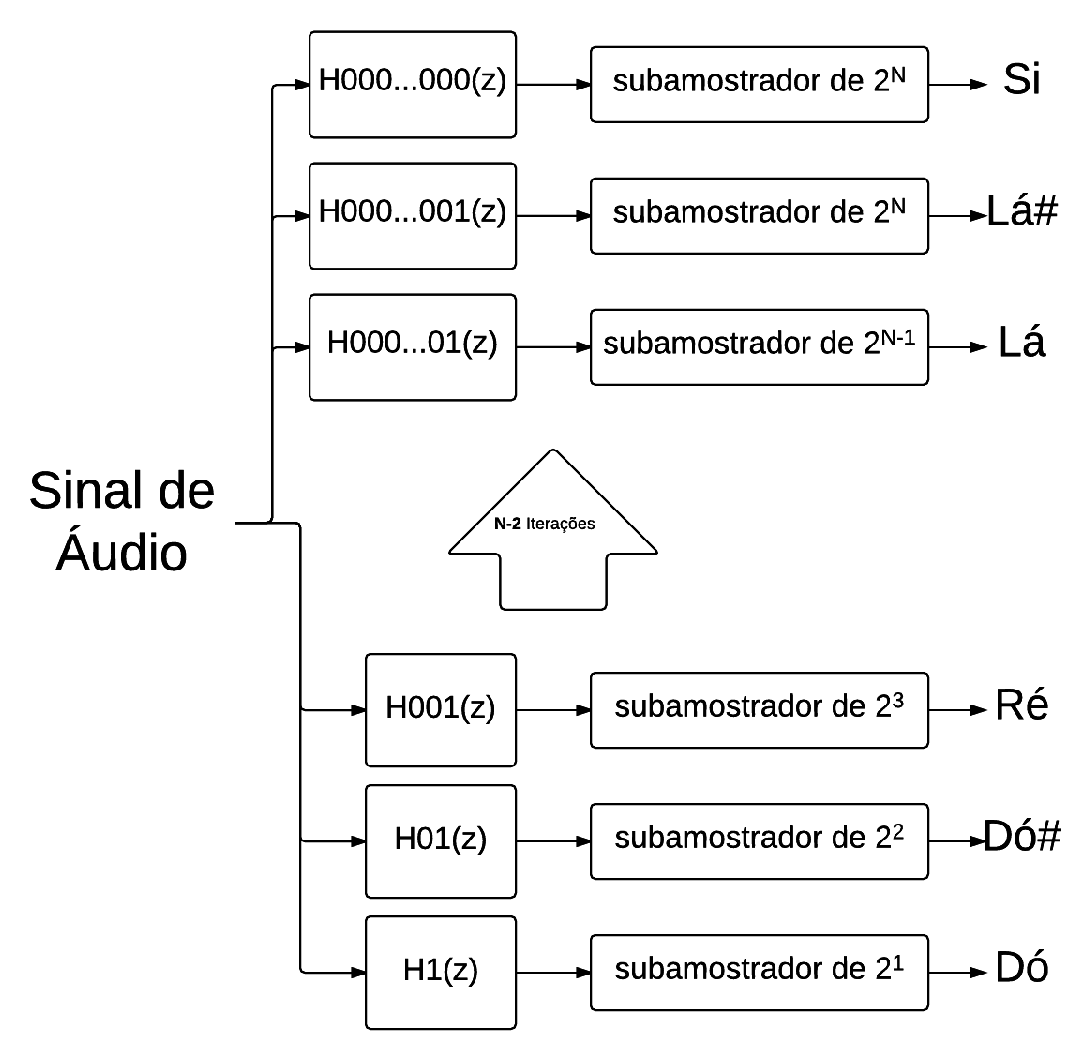
\includegraphics[keepaspectratio=true,scale=0.7]{figuras/wavelet_figura.eps}
  \caption{Hipótese ilustrativa do banco de filtros da transformada wavelets.}
  \label{fig:banco_de_filtros}
\end{figure}

Tendo em vista a figura \ref{fig:banco_de_filtros}, a hipótese é usar as iterações do banco de filtros para localizar cada nota musical nas saídas dos mesmos. Para a validação dessa hipótese usou-se wavelets da família $daubechies$ devido a alta correlação das mesmas com a natureza das ondas sonoras. Foi então verificado a viabilidade de se iterar os filtros até chegarem a resolução de uma nota musical (faixa restrita de frequências). A figura \ref{fig:440_wavelets_1} mostra o gráfico da resposta em frequência de um sinal puro de 440 Hz, oriundo da saída \textbf{H001(z)}, com o banco de filtros iterado em 3 vezes.

\begin{figure}[h]
    \centering
    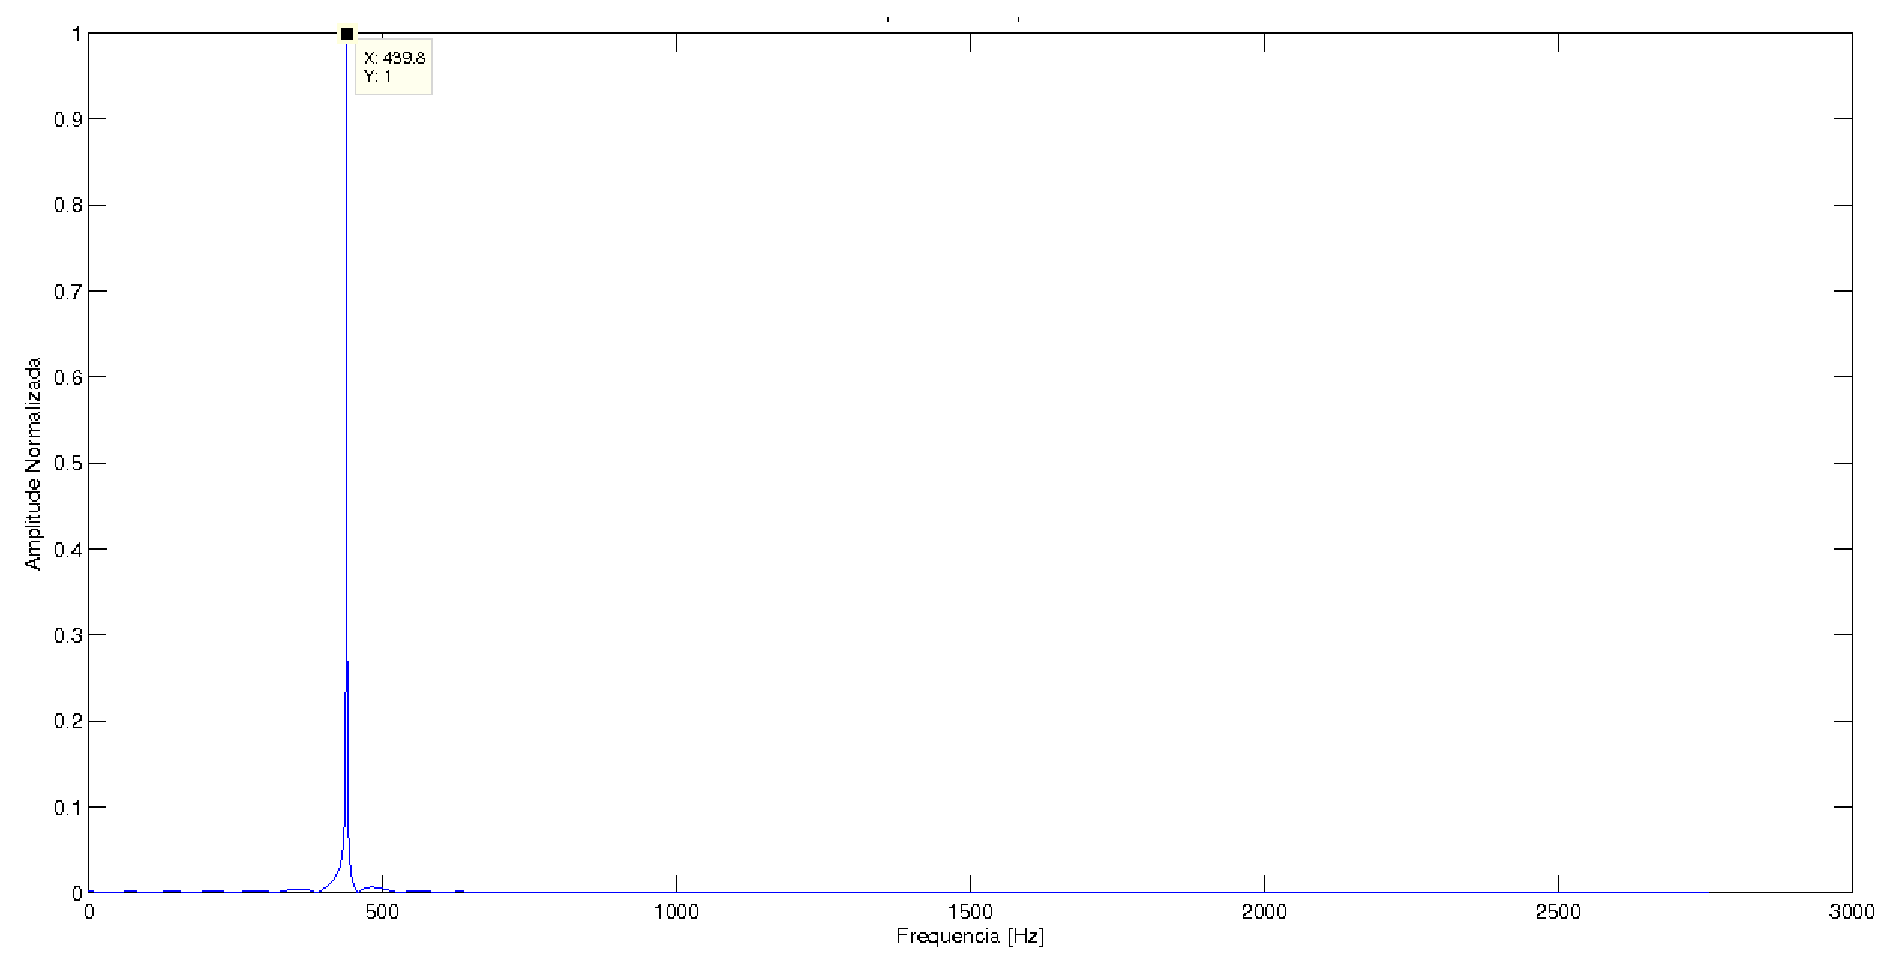
\includegraphics[keepaspectratio=true,scale=0.45]{figuras/wavelet_deslocado_1.eps}
  \caption{Gráfico da resposta em frequência de um sinal puro de 440 Hz em 3 iterações no banco de filtros.}
  \label{fig:440_wavelets_1}
\end{figure}

\newpage
De acordo com a figura \ref{fig:440_wavelets_1} é visível que em 3 iterações no banco de filtro pode se identificar a frequência em integridade de 440 Hz pelo nível de energia máximo. Porém é preciso iterar mais vezes o banco de filtros para poder isolar somente uma nota para cada saída do mesmo. A figura \ref{fig:440_wavelets_2} mostra o gráfico da resposta em frequência do mesmo sinal puro de 440 Hz, oriundo da saída \textbf{H000001(z)}, com o banco de filtros iterado em 10 vezes. Como mostra a figura \ref{fig:440_wavelets_2}, o sinal de 440 Hz na entrada do banco de filtros foi defasado para 249.4 Hz. Esse fato não corrobora com o isolamento das frequências para cada saída do banco de filtros, pois, com o aumento da iteração abordado, o sinal sofreu uma defasagem.


\begin{figure}[h]
    \centering
    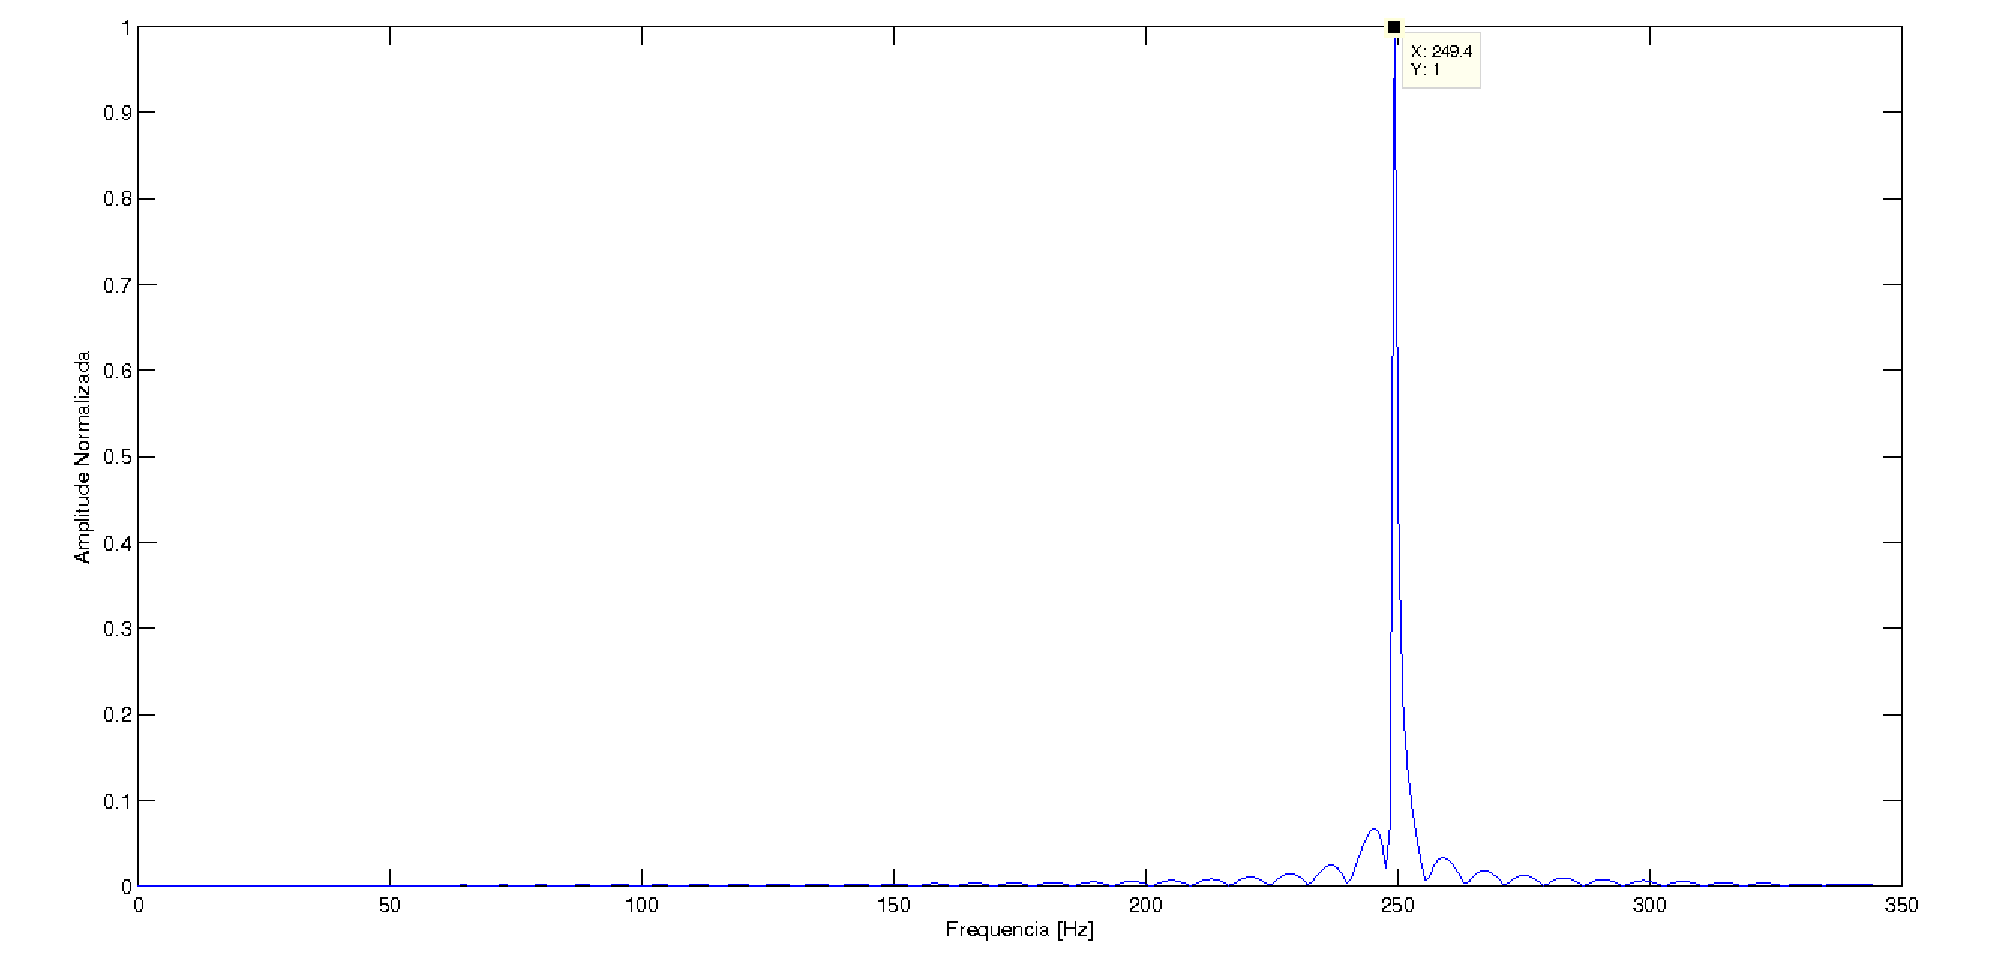
\includegraphics[keepaspectratio=true,scale=0.45]{figuras/wavelet_deslocado.eps}
  \caption{Gráfico da resposta em frequência de um sinal puro de 440 Hz em 10 iterações no banco de filtros.}
  \label{fig:440_wavelets_2}
\end{figure}

\section{Transcrição de Notas ao Longo do Tempo}
% MOSTRAR 4 CASOS DE GRAFICO DA MATRIZ DE NOTAS POR TEMPO
Dado os módulos implementados nos procedimentos \ref{subsec:procedimento_2}, \ref{subsec:procedimento_3}, \ref{subsec:procedimento_4} e \ref{subsec:procedimento_5} e os resultados dos ciclos de desenvolvimento \ref{subsec:ciclo_1}, \ref{subsec:ciclo_2}, \ref{subsec:ciclo_3}, \ref{subsec:ciclo_7} e \ref{subsec:ciclo_9}, é consolidado os resultados da transcrição automática de notas ao longo do tempo. A figura \ref{fig:notas_puras} mostra o gráfico binário de transcrição de notas de uma escala cromática, gerada a partir de um áudio de tons puros variando de 260 Hz até 520 Hz.

\begin{figure}[h]
    \centering
    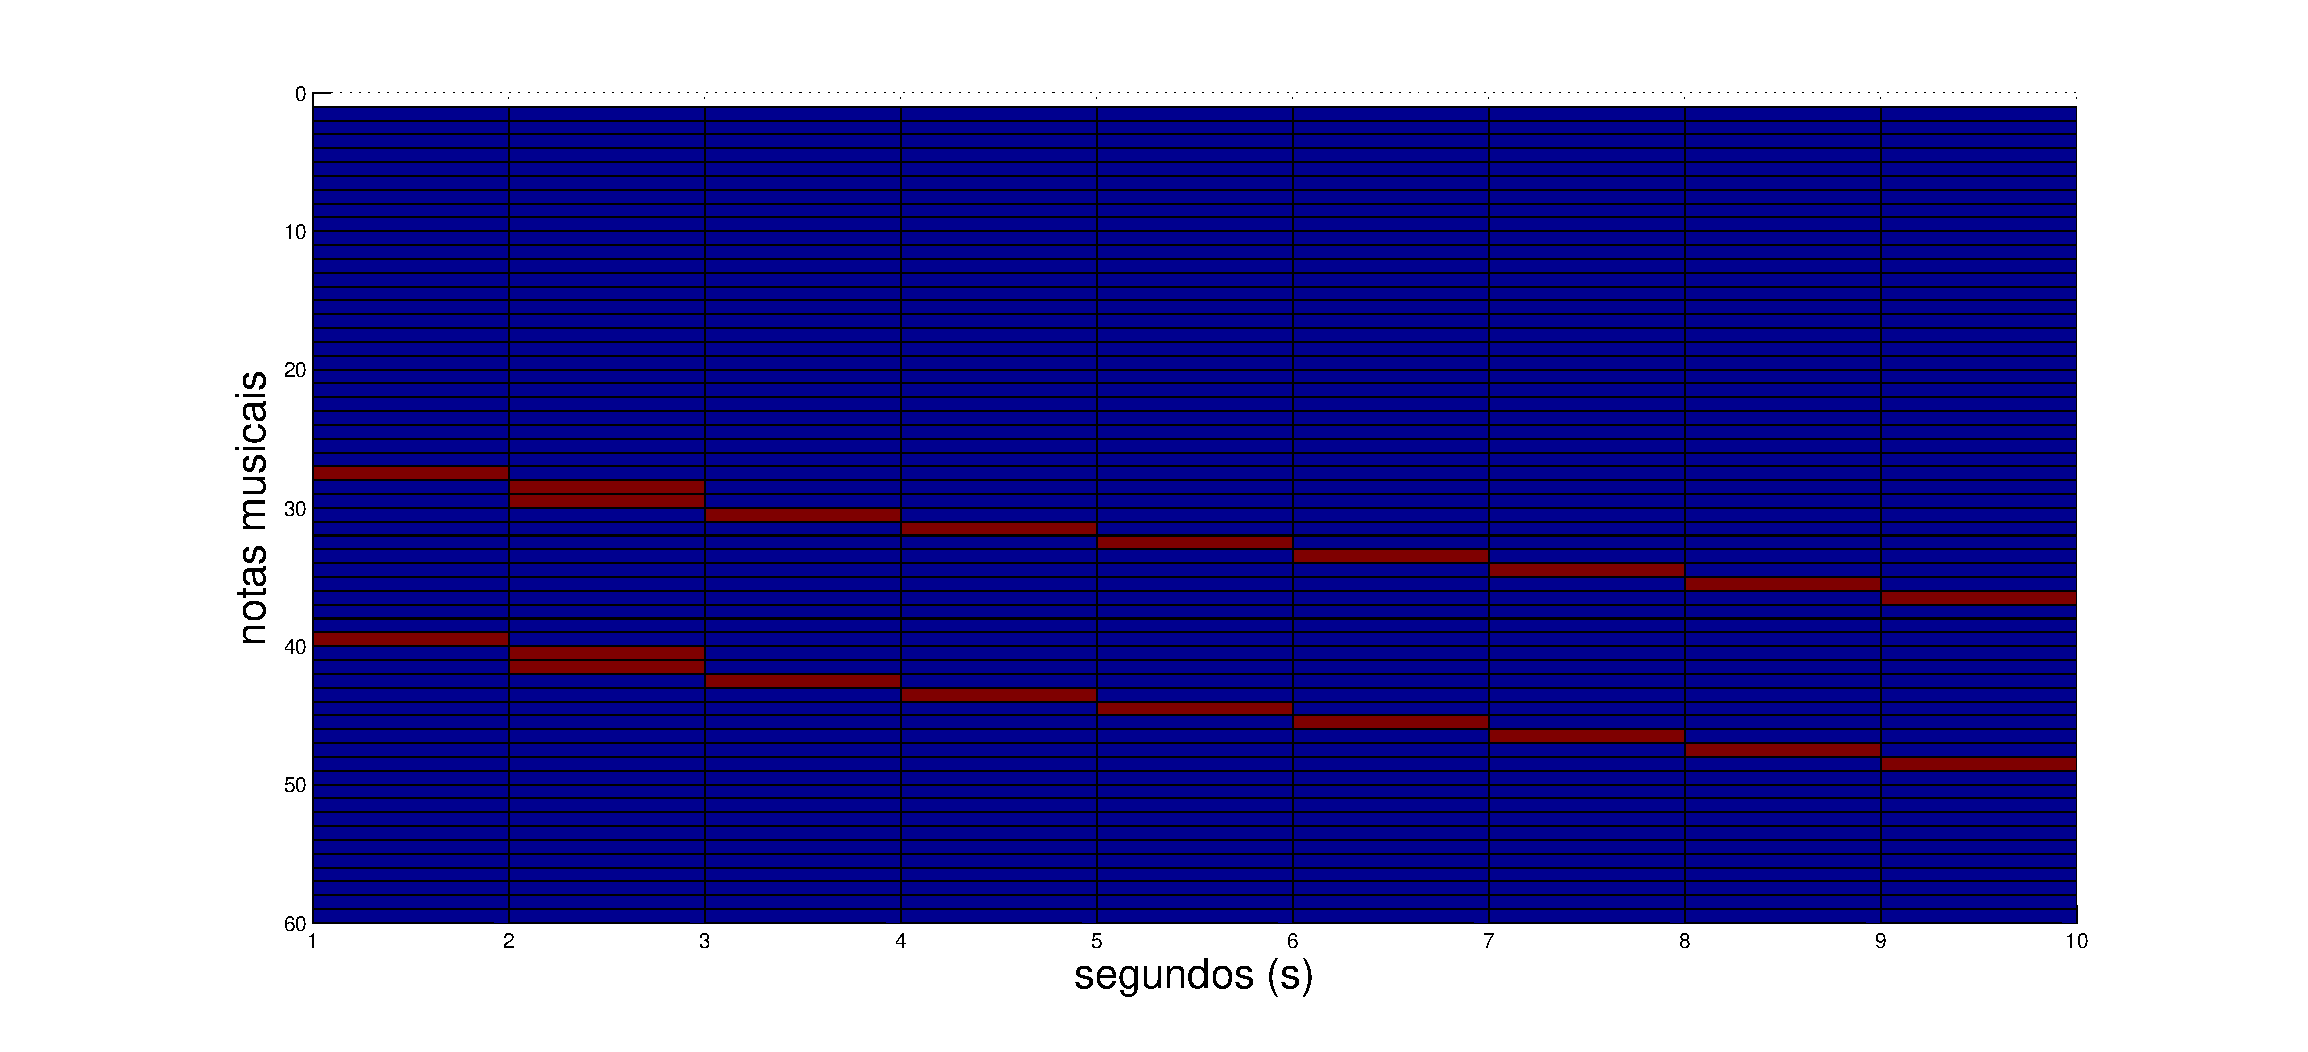
\includegraphics[keepaspectratio=true,scale=0.4]{figuras/notas_puras.eps}
  \caption{Gráfico binário de transcrição de notas a partir de um áudio de tons puros variando de 260 Hz até 520 Hz.}
  \label{fig:notas_puras}
\end{figure}       

Em vista do que é mostrado na figura \ref{fig:notas_puras}, percebe-se que não só a nota base foi reconhecida mas também o primeiro harmônico da mesma. Esse fato auxilia no reconhecimento de acordes visto que os harmônicos são prepoderantes e decivos para distinguir semitons. No que tange os aspectos de reconhecimento de notas gravadas a partir de um instrumento real, violão e piano respectivamente, as figuras \ref{fig:notas_violao} e \ref{fig:notas_piano} mostram o gráfico binário de transcrição de notas de uma escala cromática no mesmo intervalo de frequências do caso anterior.

\begin{figure}[h]
    \centering
    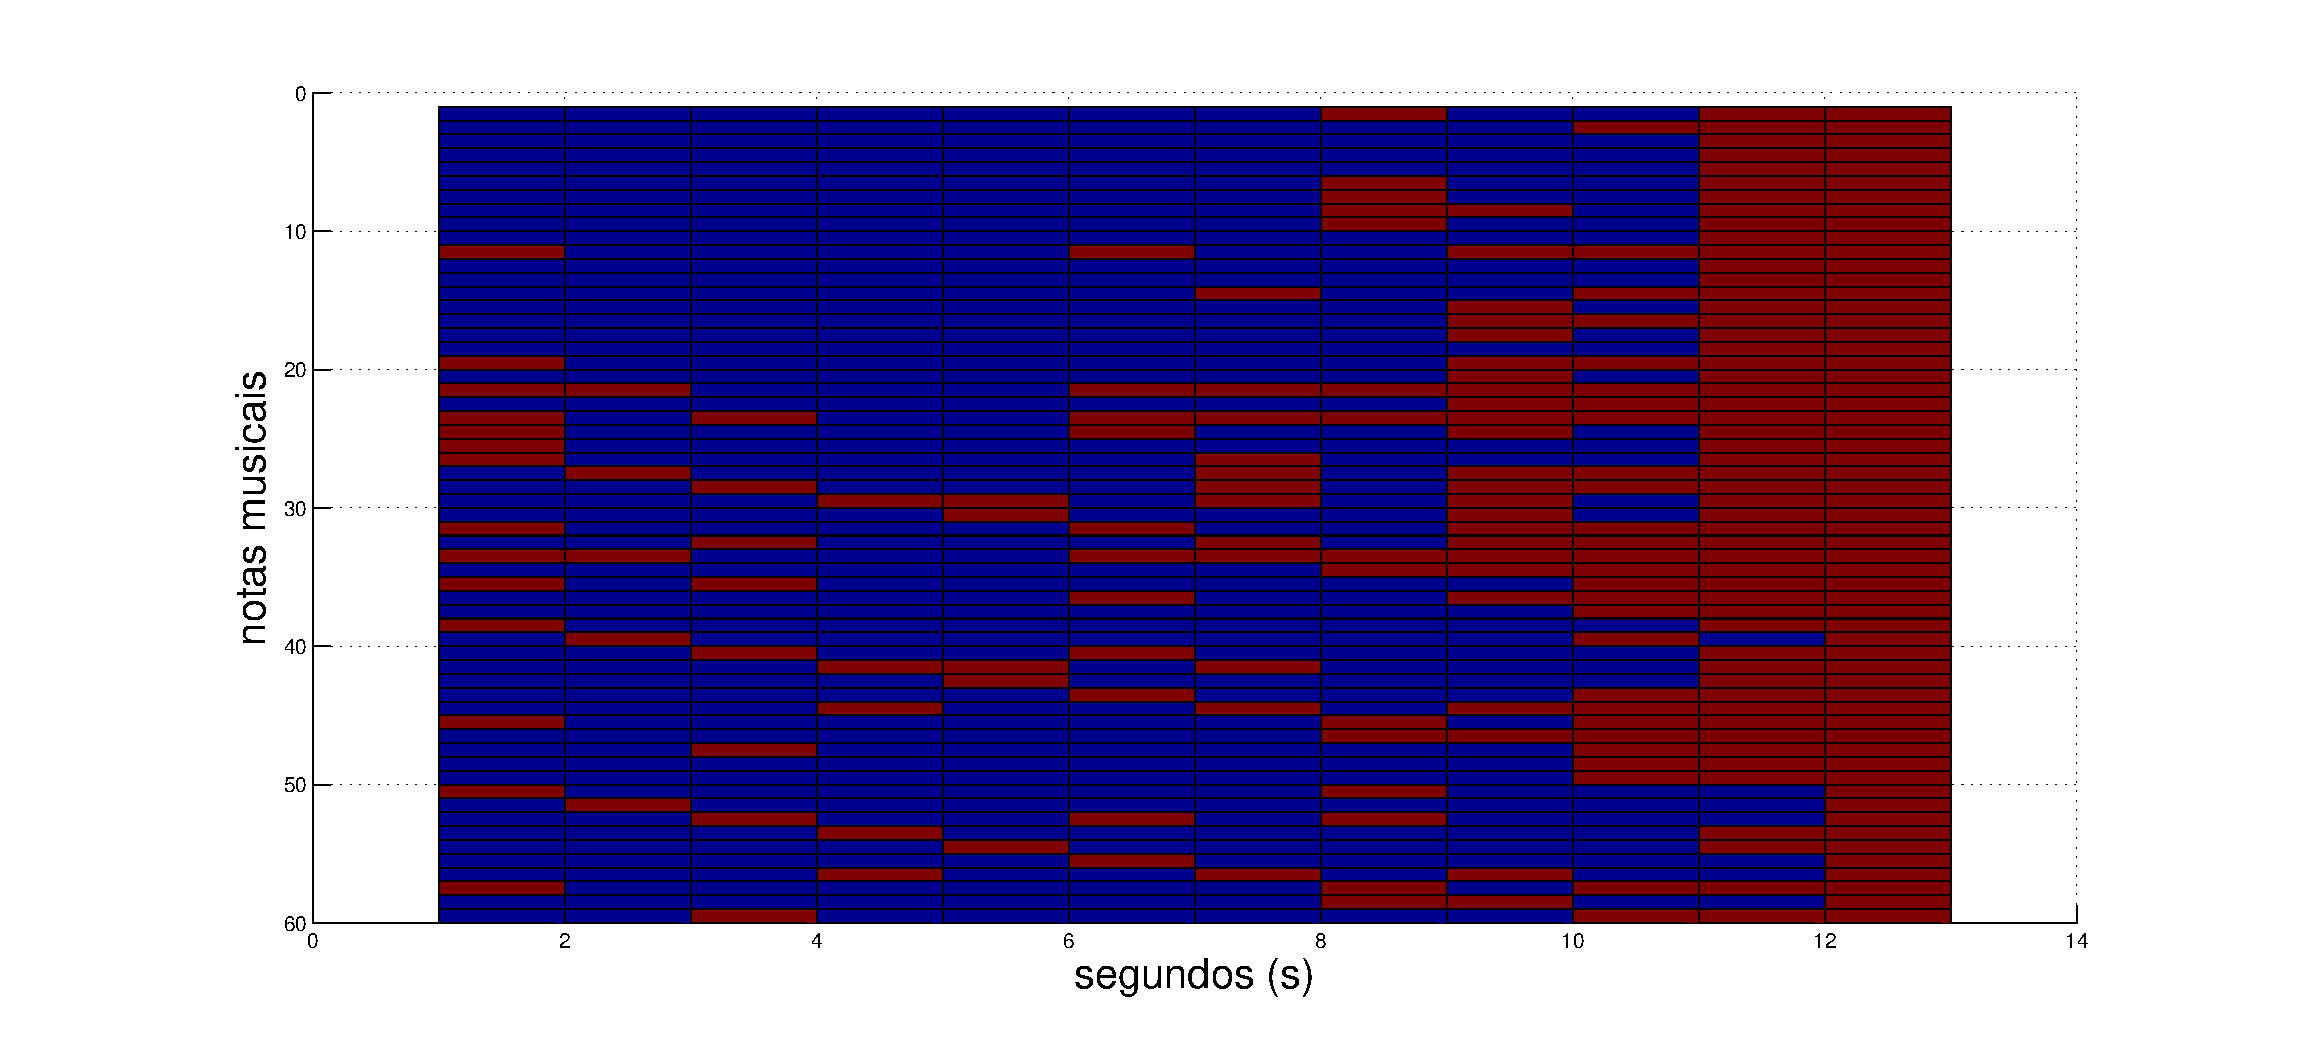
\includegraphics[keepaspectratio=true,scale=0.5]{figuras/notas_violao.eps}
  \caption{Gráfico binário de transcrição de notas a partir de um áudio de tons de violão variando de 260 Hz até 520 Hz.}
  \label{fig:notas_violao}
\end{figure}       

Dado a figura \ref{fig:notas_violao}, é perceptível uma escala gradual de semitons de violão junto com notas de ruídos de fundo. Cada nota e cada ruído de fundo gera um harmônico ocasionando em notas que não estão presentes efetivamente no áudio.

Dado a figura \ref{fig:notas_piano}, é perceptível, com mais clareza em relação ao violão, uma escala gradual de semitons de piano. Cada nota gerou também seus respectivos harmônicos mesmo em escala inferior ao do violão.

Mesmo nos contextos de erros de ruídos de fundos mostrados nas figuras anteriores, a rede neural minimiza-os através de padrões de tríades oriundos da teoria musical de acordes.

\begin{figure}[h]
    \centering
    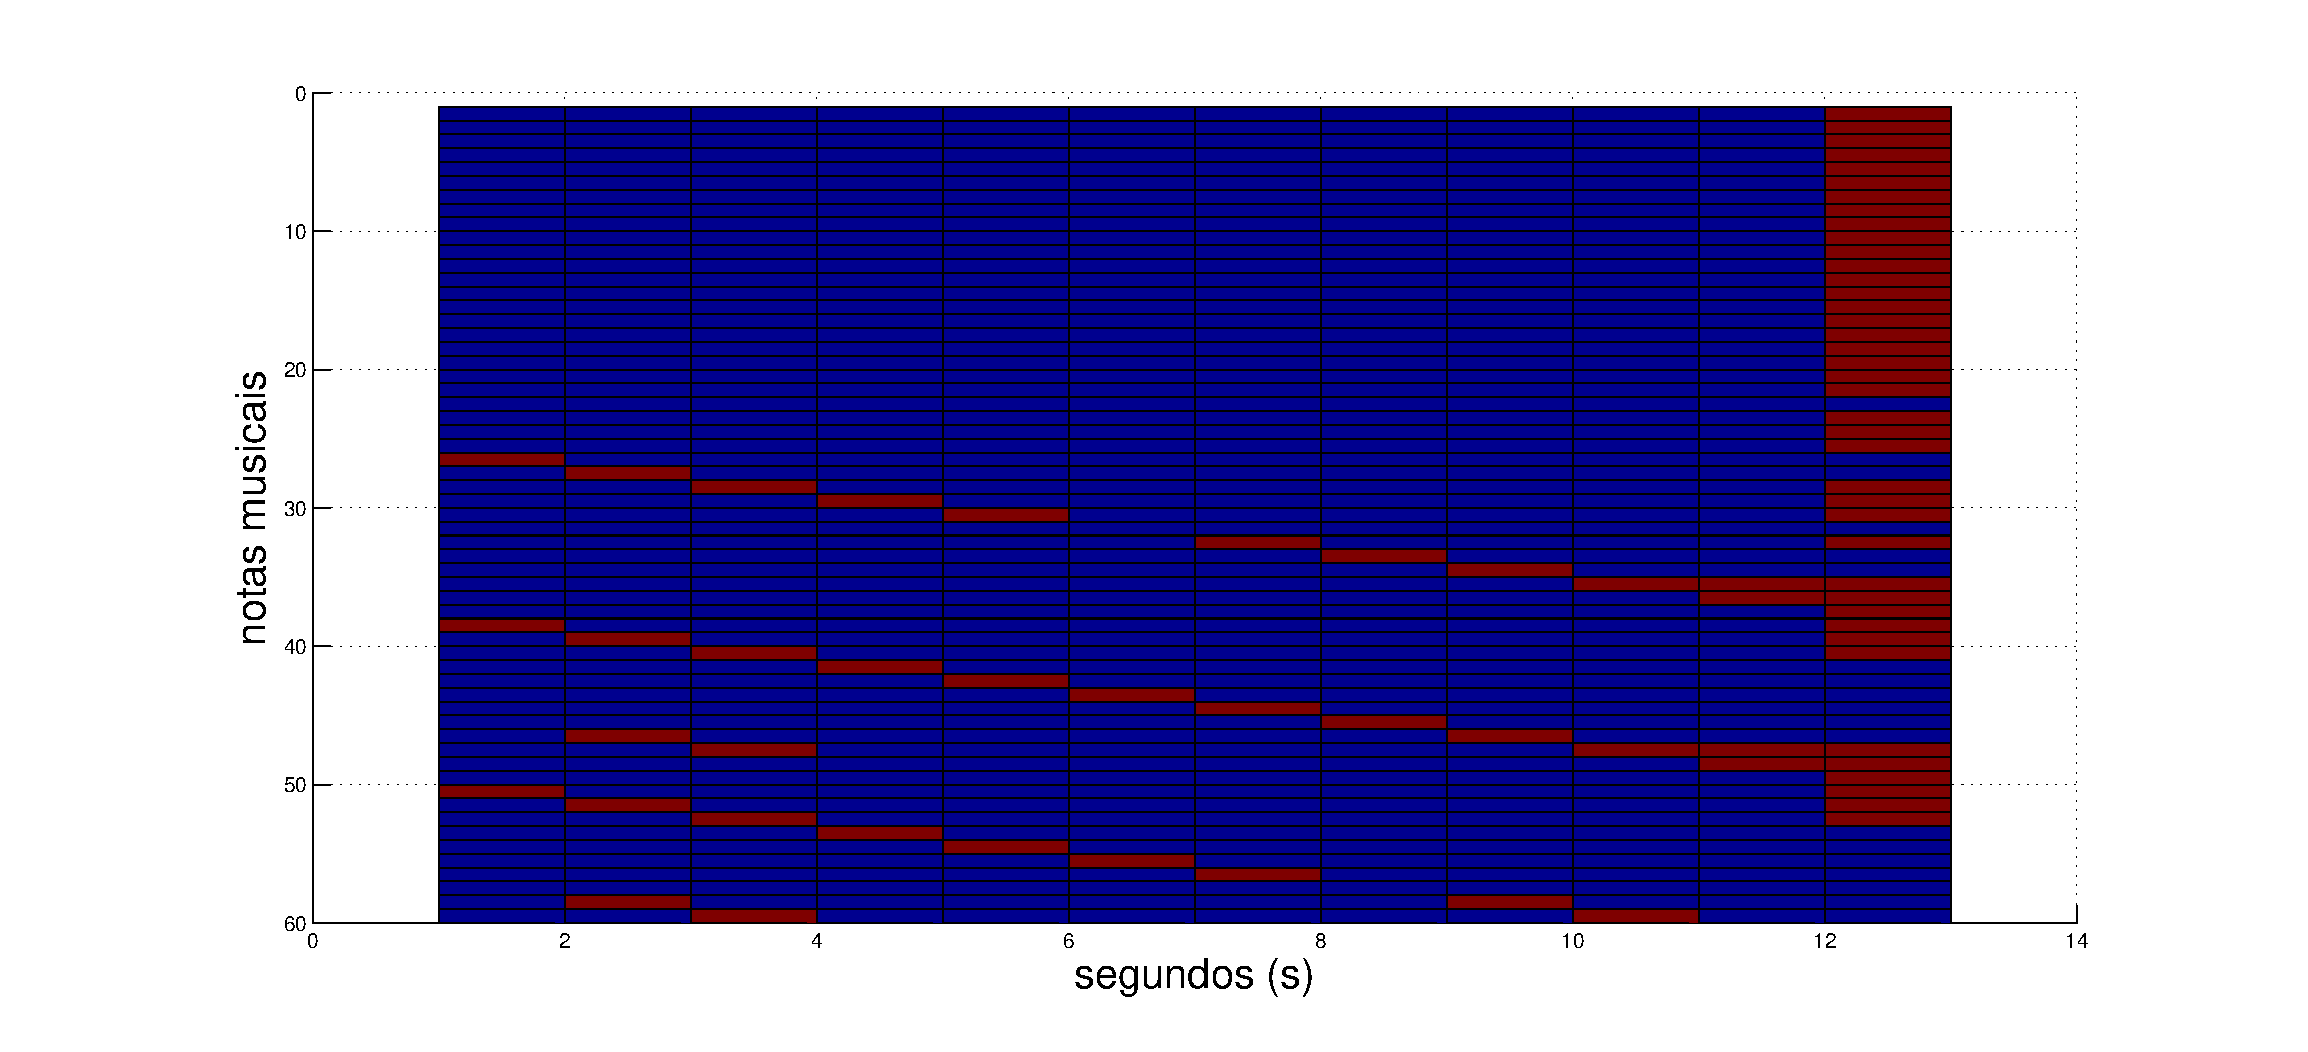
\includegraphics[keepaspectratio=true,scale=0.5]{figuras/notas_piano.eps}
  \caption{Gráfico binário de transcrição de notas a partir de um áudio de tons de piano variando de 260 Hz até 520 Hz.}
  \label{fig:notas_piano}
\end{figure}


\section{Transcrição Automática de Acordes ao Longo do Tempo}
% MOSTRAR 4 CASOS DE LINHAS DE ACORDES NO TEMPO
Tendo como referência os módulos implementados nos procedimentos \ref{subsec:procedimento_1}, \ref{subsec:procedimento_2}, \ref{subsec:procedimento_3}, \ref{subsec:procedimento_4}, \ref{subsec:procedimento_5}, \ref{subsec:procedimento_6}, \ref{subsec:procedimento_8}, \ref{subsec:procedimento_9} e \ref{subsec:procedimento_10} e os resultados dos ciclos de desenvolvimento \ref{subsec:ciclo_1}, \ref{subsec:ciclo_2}, \ref{subsec:ciclo_3}, \ref{subsec:ciclo_4}, \ref{subsec:ciclo_7}, \ref{subsec:ciclo_9}, \ref{subsec:ciclo_9}, \ref{subsec:ciclo_10}, \ref{subsec:ciclo_11} e \ref{subsec:ciclo_12}, é consolidado os resultados da transcrição automática de acordes ao longo do tempo. Foi feito 2 experimentos testando a sequência de acordes tocados no piano e no violão. A figura \ref{fig:acordes_piano} mostra o sinal de áudio do piano.

\begin{figure}[h]
    \centering
    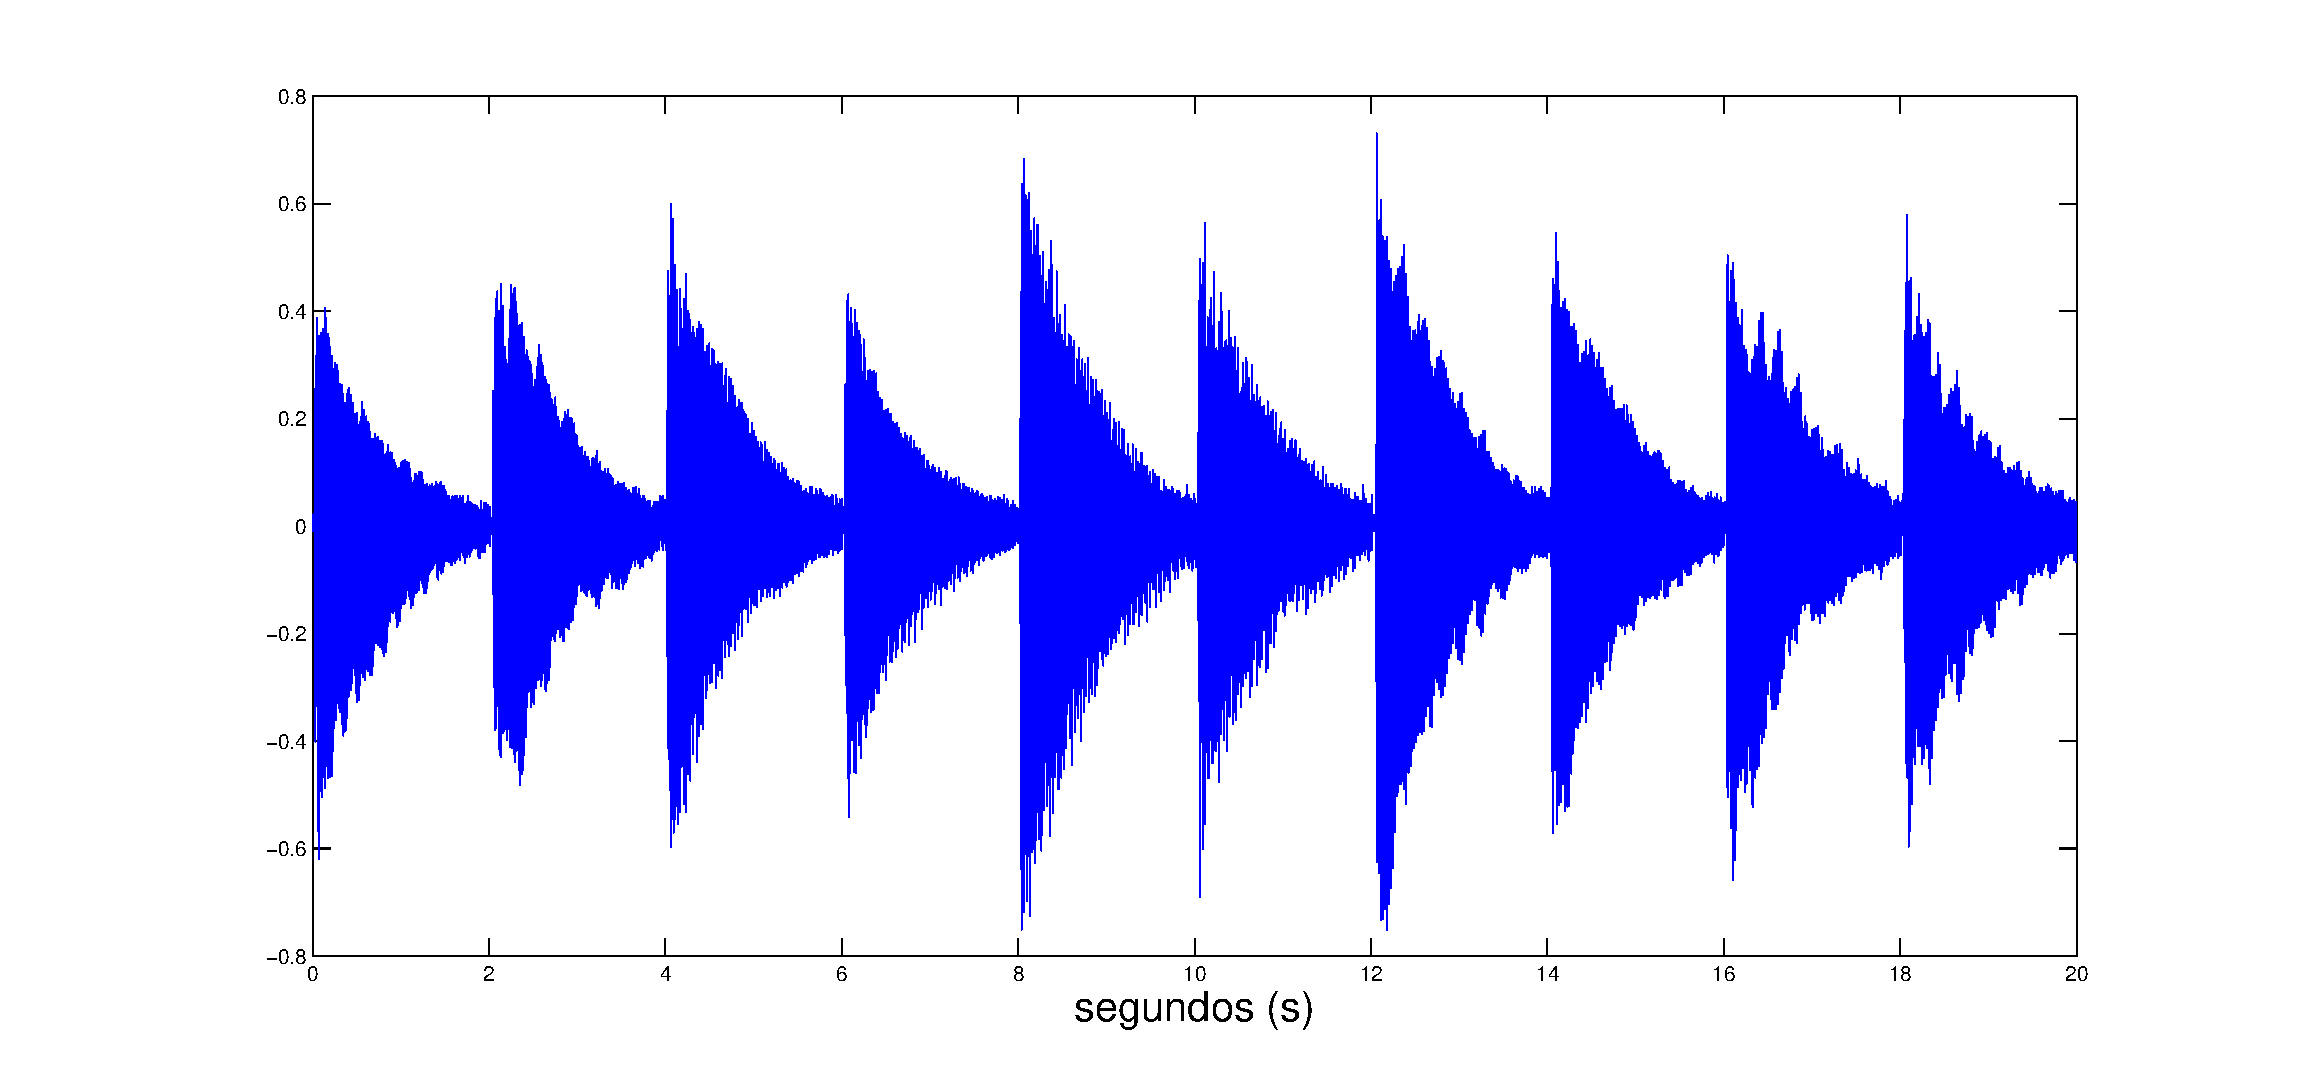
\includegraphics[keepaspectratio=true,scale=0.3]{figuras/acordes_piano.eps}
  \caption{Gráfico do sinal de áudio do piano.}
  \label{fig:acordes_piano}
\end{figure}


Como é visível na figura \ref{fig:acordes_piano}, há 10 acordes tocados ao longo de aproximadamente 20 sengudos e cada acorde foi executado aproximadamente durante 2 segundos. A tabela \ref{tab:acordes_piano} mostra o momento, acordes tocados e os acordes reconhecidos pelo sistema.

\begin{table}[h]
\centering
    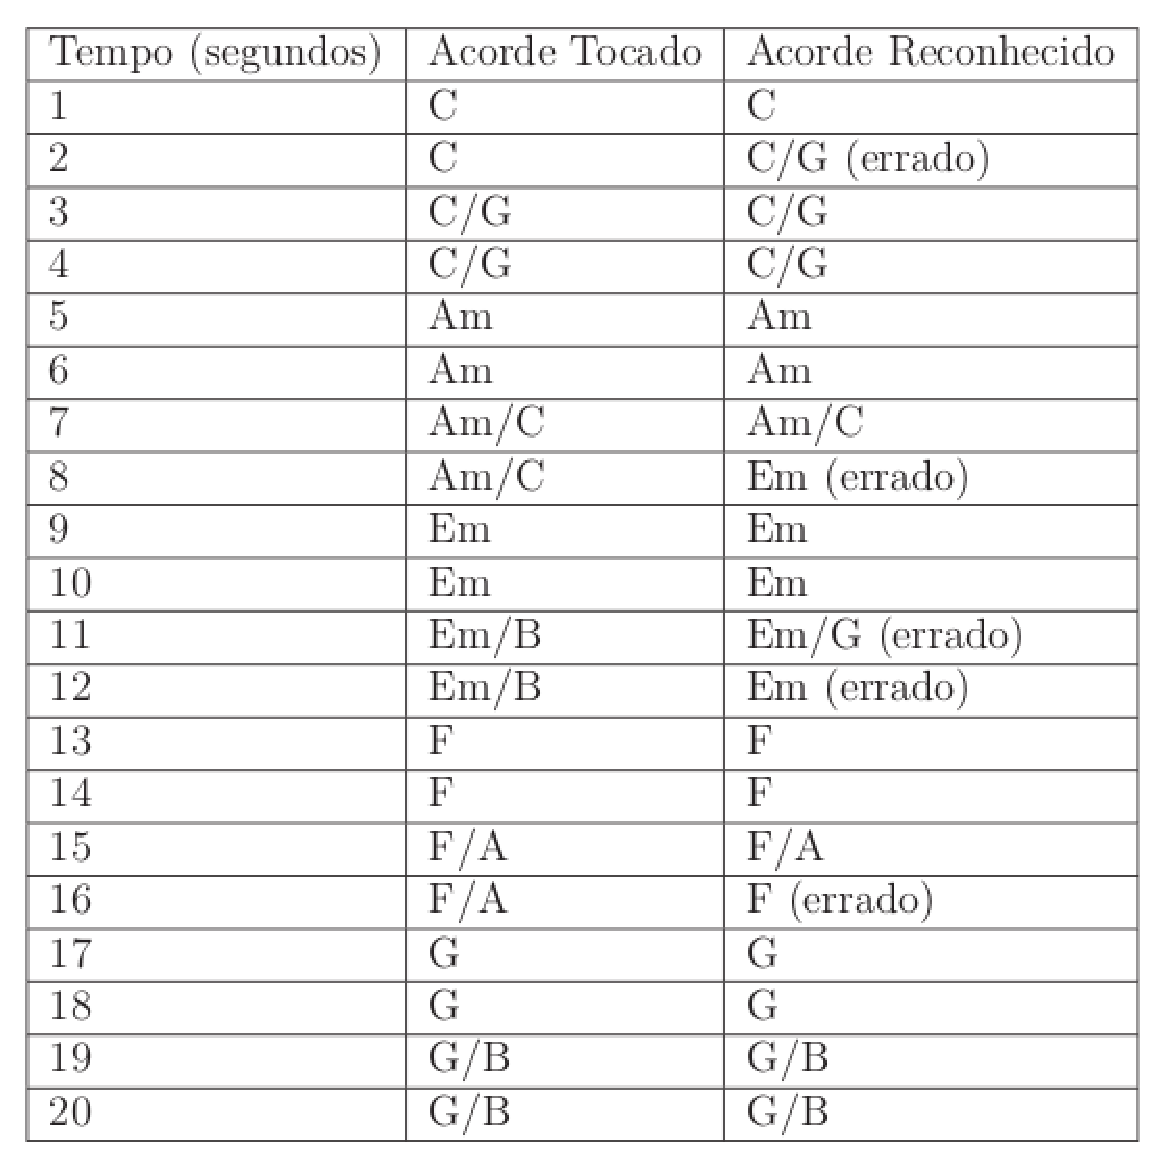
\includegraphics[keepaspectratio=true,scale=0.5]{figuras/tabela_acordes_piano.eps}
  \caption{Tabela de acordes tocados e acordes reconhecidos no piano.}
  \label{tab:acordes_piano}
\end{table}

Da tabela \ref{tab:acordes_piano} pode-se ver os acordes que a solução computacional errou totalizando em 5 acordes. Dentre 20 acordes tocados em sequência o sistema acertou 15, ocasionando em 75\% de acertos.

Também foi feito o mesmo experimento com o sinal de áudio de violão, sendo representado pela figura \ref{fig:acordes_violao}. Como foi feito também com o piano, são no total 10 acordes, cada um com duração de 2 segundos totalizando num sinal de 20 segundos aproximadamente.

\begin{figure}[h]
    \centering
    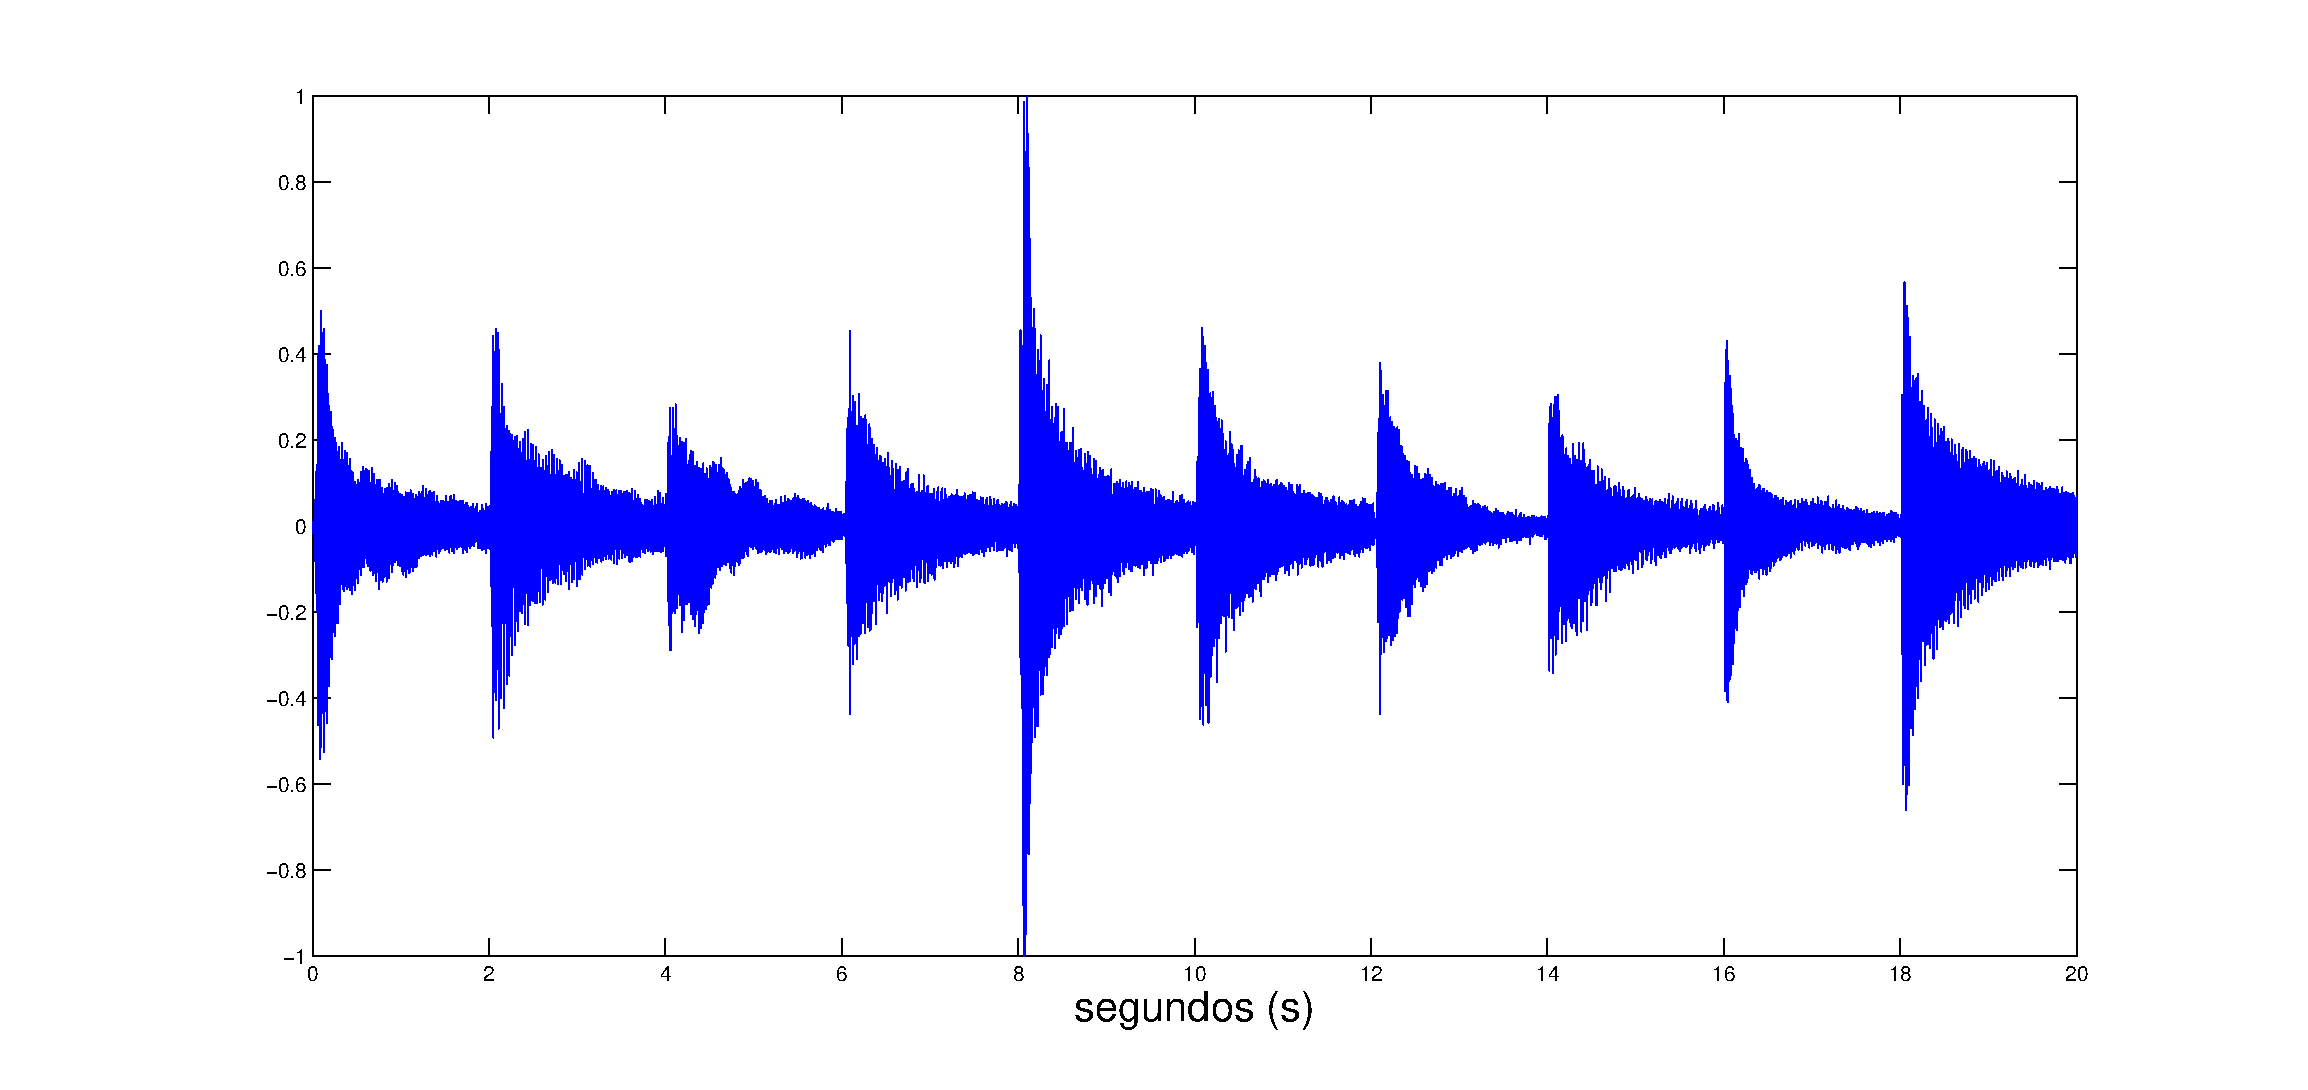
\includegraphics[keepaspectratio=true,scale=0.3]{figuras/acordes_violao.eps}
  \caption{Gráfico do sinal de áudio do violão.}
  \label{fig:acordes_violao}
\end{figure}

Também é evidenciado na tabela \ref{tab:acordes_violao} os acordes tocados e os acordes reconhecidos no violão. O sistema reconheceu incorretamente 10 acordes de 20, totalizando 50\% de acertos no violão.

\begin{table}[h]
\centering
    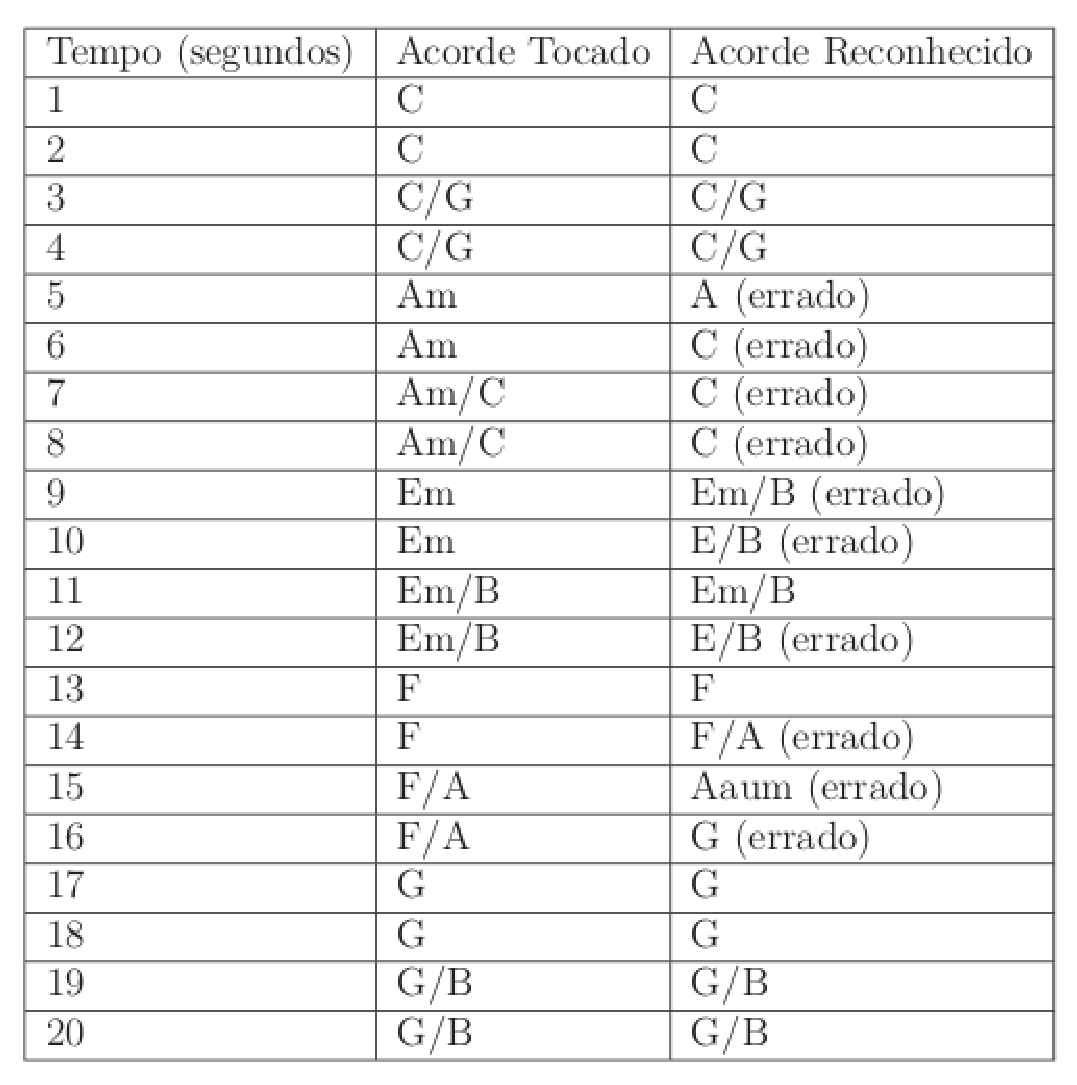
\includegraphics[keepaspectratio=true,scale=0.5]{figuras/tabela_acordes_violao.eps}
  \caption{Tabela de acordes tocados e acordes reconhecidos no violão.}
  \label{tab:acordes_violao}
\end{table}


\section{Extração da Tonalidade}
% MOSTRAR 4 EXEMPLOS DE LINHAS DE ACORDES E O TOM

A extração da tonalidade das músicas foi consolidada de acordo com os procedimentos \ref{subsec:procedimento_1}, \ref{subsec:procedimento_2}, \ref{subsec:procedimento_3}, \ref{subsec:procedimento_4}, \ref{subsec:procedimento_5}, \ref{subsec:procedimento_6} e \ref{subsec:procedimento_7} e ciclos de desenvolvimento \ref{subsec:ciclo_1}, \ref{subsec:ciclo_2}, \ref{subsec:ciclo_3}, \ref{subsec:ciclo_4}, \ref{subsec:ciclo_8} e \ref{subsec:ciclo_9}. Para validar a extração do tom da música foi feito 6 experimentos com 4 músicas completas e diferentes e 2 sequências de acordes iguais porém com instrumentos diferentes (sequências essas oriundas do caso abordado de extração de acordes ao longo do tempo). A tabela \ref{tab:tons} mostra o resultados dos experimentos em relação ao tom de fato da música\footnote{Os tons das músicas que não foram tocadas manualmente foram tirados do site http://www.cifraclub.com.br/} e tom reconhecimento pelo sistema.

\begin{table}[h]
\centering
\begin{tabular}{|l|l|l|}
\hline
Musica                           & Tom da Música & Tom Reconhecido \\ \hline
Sequência de Acordes no Piano    & C             & C               \\ \hline
Sequência de Acordes no Violão   & C             & Em (errado)     \\ \hline
The Beatles - Oh Darling         & A             & A               \\ \hline
Deep Purple - Smoke on the Water & Gm            & G (errado)      \\ \hline
Legião Urbana - Eduardo e Mônica & E             & E               \\ \hline
The Beatles - Yesterday          & F             & F               \\ \hline
\end{tabular}
\label{tab:tons}
\end{table}

Diante do que é mostrado na tabela \ref{tab:tons}, o sistema errou 2 músicas de 6 músicas no total, ocasionando em 67\% de acertos globais.

